% Options for packages loaded elsewhere
\PassOptionsToPackage{unicode}{hyperref}
\PassOptionsToPackage{hyphens}{url}
%
\documentclass[
]{article}
\usepackage{lmodern}
\usepackage{amssymb,amsmath}
\usepackage{ifxetex,ifluatex}
\ifnum 0\ifxetex 1\fi\ifluatex 1\fi=0 % if pdftex
  \usepackage[T1]{fontenc}
  \usepackage[utf8]{inputenc}
  \usepackage{textcomp} % provide euro and other symbols
\else % if luatex or xetex
  \usepackage{unicode-math}
  \defaultfontfeatures{Scale=MatchLowercase}
  \defaultfontfeatures[\rmfamily]{Ligatures=TeX,Scale=1}
\fi
% Use upquote if available, for straight quotes in verbatim environments
\IfFileExists{upquote.sty}{\usepackage{upquote}}{}
\IfFileExists{microtype.sty}{% use microtype if available
  \usepackage[]{microtype}
  \UseMicrotypeSet[protrusion]{basicmath} % disable protrusion for tt fonts
}{}
\makeatletter
\@ifundefined{KOMAClassName}{% if non-KOMA class
  \IfFileExists{parskip.sty}{%
    \usepackage{parskip}
  }{% else
    \setlength{\parindent}{0pt}
    \setlength{\parskip}{6pt plus 2pt minus 1pt}}
}{% if KOMA class
  \KOMAoptions{parskip=half}}
\makeatother
\usepackage{xcolor}
\IfFileExists{xurl.sty}{\usepackage{xurl}}{} % add URL line breaks if available
\IfFileExists{bookmark.sty}{\usepackage{bookmark}}{\usepackage{hyperref}}
\hypersetup{
  pdftitle={Supplementary},
  hidelinks,
  pdfcreator={LaTeX via pandoc}}
\urlstyle{same} % disable monospaced font for URLs
\usepackage[margin=1in]{geometry}
\usepackage{longtable,booktabs}
% Correct order of tables after \paragraph or \subparagraph
\usepackage{etoolbox}
\makeatletter
\patchcmd\longtable{\par}{\if@noskipsec\mbox{}\fi\par}{}{}
\makeatother
% Allow footnotes in longtable head/foot
\IfFileExists{footnotehyper.sty}{\usepackage{footnotehyper}}{\usepackage{footnote}}
\makesavenoteenv{longtable}
\usepackage{graphicx,grffile}
\makeatletter
\def\maxwidth{\ifdim\Gin@nat@width>\linewidth\linewidth\else\Gin@nat@width\fi}
\def\maxheight{\ifdim\Gin@nat@height>\textheight\textheight\else\Gin@nat@height\fi}
\makeatother
% Scale images if necessary, so that they will not overflow the page
% margins by default, and it is still possible to overwrite the defaults
% using explicit options in \includegraphics[width, height, ...]{}
\setkeys{Gin}{width=\maxwidth,height=\maxheight,keepaspectratio}
% Set default figure placement to htbp
\makeatletter
\def\fps@figure{htbp}
\makeatother
\setlength{\emergencystretch}{3em} % prevent overfull lines
\providecommand{\tightlist}{%
  \setlength{\itemsep}{0pt}\setlength{\parskip}{0pt}}
\setcounter{secnumdepth}{-\maxdimen} % remove section numbering
\usepackage{booktabs}
\usepackage{longtable}
\usepackage{array}
\usepackage{multirow}
\usepackage{wrapfig}
\usepackage{float}
\usepackage{colortbl}
\usepackage{pdflscape}
\usepackage{tabu}
\usepackage{threeparttable}
\usepackage{threeparttablex}
\usepackage[normalem]{ulem}
\usepackage{makecell}
\usepackage{xcolor}

\title{Supplementary}
\author{}
\date{\vspace{-2.5em}}

\begin{document}
\maketitle

\emph{Epigenetic and genetic population structure is coupled in a marine
invertebrate}\\
Katherine Silliman, Laura H Spencer, Sam White, Steven B Roberts

\hypertarget{general-o.-lurida-methylation-characteristics}{%
\subsubsection{\texorpdfstring{1. General \emph{O. lurida} methylation
characteristics}{1. General O. lurida methylation characteristics}}\label{general-o.-lurida-methylation-characteristics}}

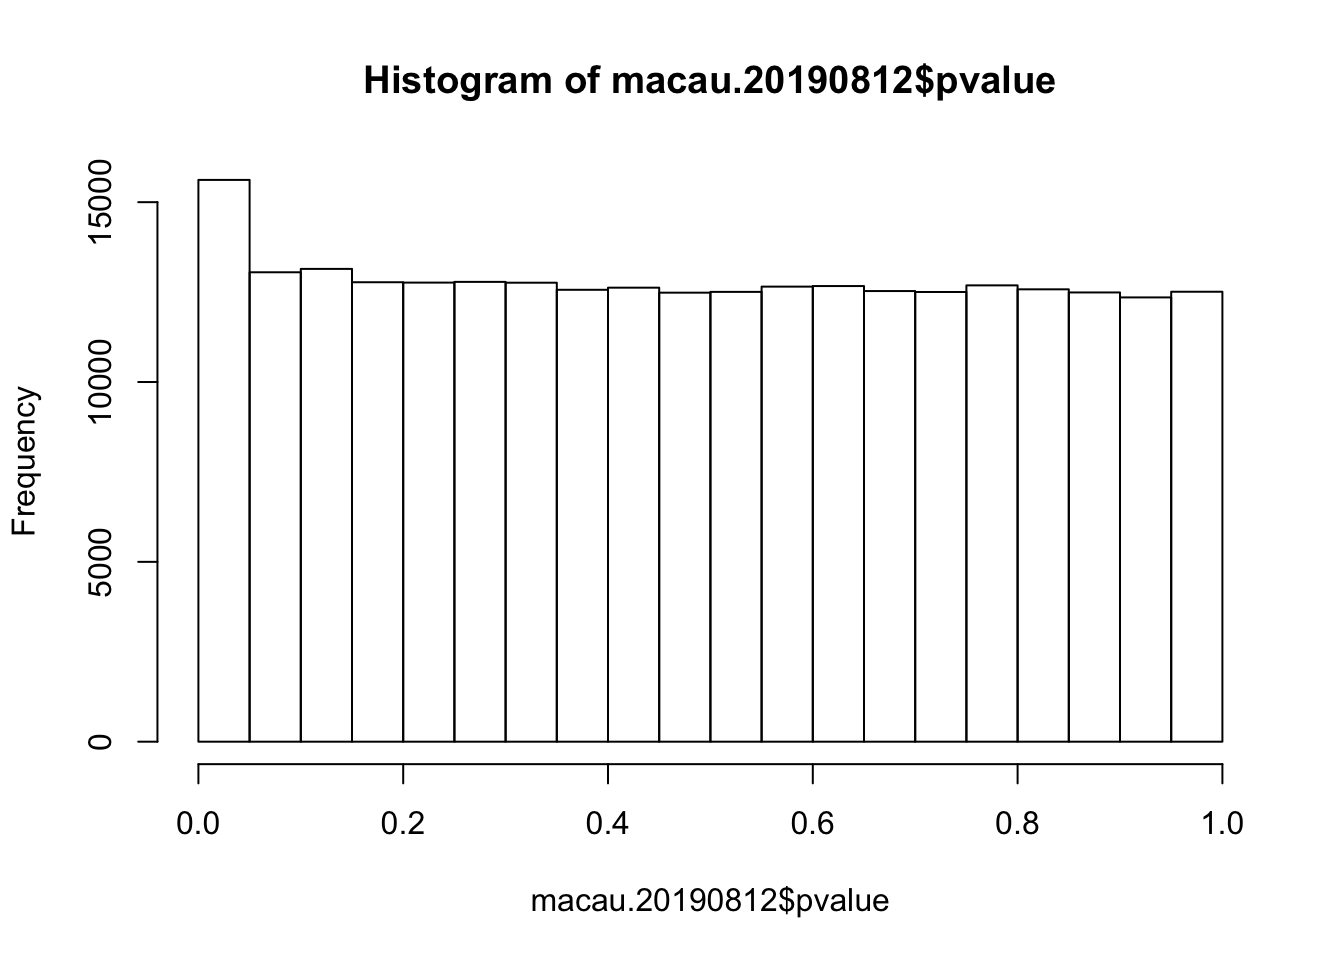
\includegraphics{Supplementary_files/figure-latex/unnamed-chunk-2-1.pdf}

\textbf{Supplemental Figure 1}: Frequency distribution of \% methylation
in \emph{O. lurida} prior to filtering (left) and after filtering for
loci with at minimum 5x coverage (right).

\begin{center}\rule{0.5\linewidth}{0.5pt}\end{center}

\begin{longtable}[]{@{}llll@{}}
\toprule
\begin{minipage}[b]{0.22\columnwidth}\raggedright
Feature\strut
\end{minipage} & \begin{minipage}[b]{0.22\columnwidth}\raggedright
\% of all CpGs in genome\strut
\end{minipage} & \begin{minipage}[b]{0.22\columnwidth}\raggedright
\% of all methylated loci\strut
\end{minipage} & \begin{minipage}[b]{0.22\columnwidth}\raggedright
Ratio of \% meth:\%CpG\strut
\end{minipage}\tabularnewline
\midrule
\endhead
\begin{minipage}[t]{0.22\columnwidth}\raggedright
Exon\strut
\end{minipage} & \begin{minipage}[t]{0.22\columnwidth}\raggedright
3.99\%\strut
\end{minipage} & \begin{minipage}[t]{0.22\columnwidth}\raggedright
14.71\%\strut
\end{minipage} & \begin{minipage}[t]{0.22\columnwidth}\raggedright
3.69\strut
\end{minipage}\tabularnewline
\begin{minipage}[t]{0.22\columnwidth}\raggedright
Intron\strut
\end{minipage} & \begin{minipage}[t]{0.22\columnwidth}\raggedright
13.94\%\strut
\end{minipage} & \begin{minipage}[t]{0.22\columnwidth}\raggedright
19.76\%\strut
\end{minipage} & \begin{minipage}[t]{0.22\columnwidth}\raggedright
1.42\strut
\end{minipage}\tabularnewline
\begin{minipage}[t]{0.22\columnwidth}\raggedright
5' flanking region (-2kb)\strut
\end{minipage} & \begin{minipage}[t]{0.22\columnwidth}\raggedright
3.91\%\strut
\end{minipage} & \begin{minipage}[t]{0.22\columnwidth}\raggedright
4.64\%\strut
\end{minipage} & \begin{minipage}[t]{0.22\columnwidth}\raggedright
1.19\strut
\end{minipage}\tabularnewline
\begin{minipage}[t]{0.22\columnwidth}\raggedright
3' flanking region (+2kb)\strut
\end{minipage} & \begin{minipage}[t]{0.22\columnwidth}\raggedright
3.92\%\strut
\end{minipage} & \begin{minipage}[t]{0.22\columnwidth}\raggedright
4.66\%\strut
\end{minipage} & \begin{minipage}[t]{0.22\columnwidth}\raggedright
1.19\strut
\end{minipage}\tabularnewline
\begin{minipage}[t]{0.22\columnwidth}\raggedright
Transposable Elements\strut
\end{minipage} & \begin{minipage}[t]{0.22\columnwidth}\raggedright
14.93\%\strut
\end{minipage} & \begin{minipage}[t]{0.22\columnwidth}\raggedright
13.83\%\strut
\end{minipage} & \begin{minipage}[t]{0.22\columnwidth}\raggedright
0.93\strut
\end{minipage}\tabularnewline
\begin{minipage}[t]{0.22\columnwidth}\raggedright
Unknown genome regions\strut
\end{minipage} & \begin{minipage}[t]{0.22\columnwidth}\raggedright
56.01\%\strut
\end{minipage} & \begin{minipage}[t]{0.22\columnwidth}\raggedright
32.25\%\strut
\end{minipage} & \begin{minipage}[t]{0.22\columnwidth}\raggedright
0.58\strut
\end{minipage}\tabularnewline
\bottomrule
\end{longtable}

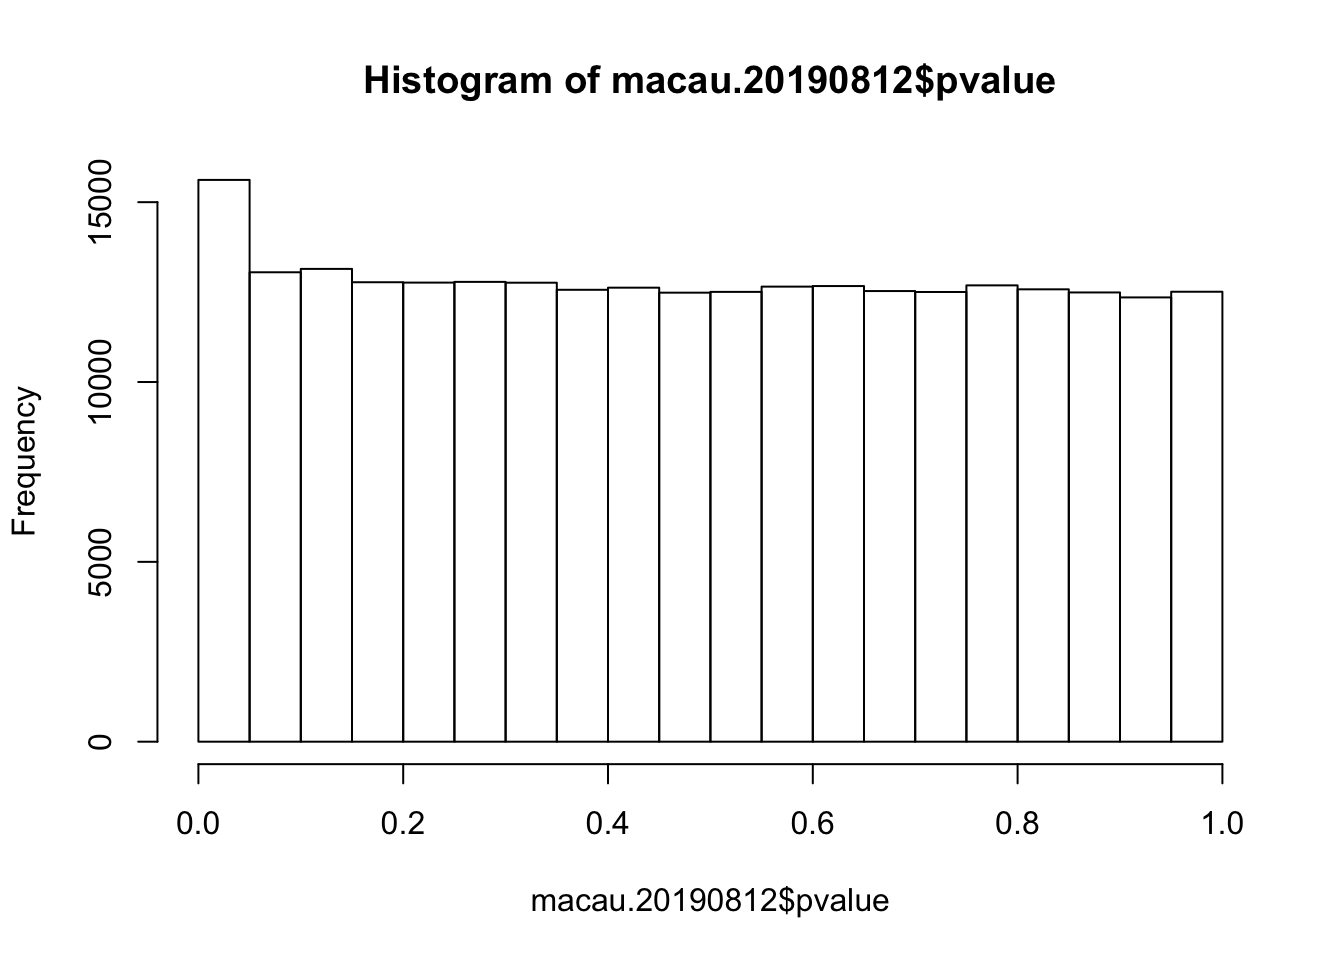
\includegraphics{Supplementary_files/figure-latex/unnamed-chunk-3-1.pdf}

\textbf{Supplemental Figure 2}: Top: Table showing the \% of all CpG
loci and methylated loci that overlap with each genomic feature. Bottom:
A correlation plot, showing residuals from chi-squared tests of
homogeneity on the distribution of methylated loci and CpG loci that
intersect with features. Blue=positive associations, red=negative
associations, and size of circles represents the absolute value of each
correlation coefficient.

\begin{center}\rule{0.5\linewidth}{0.5pt}\end{center}

\begin{figure}
\centering
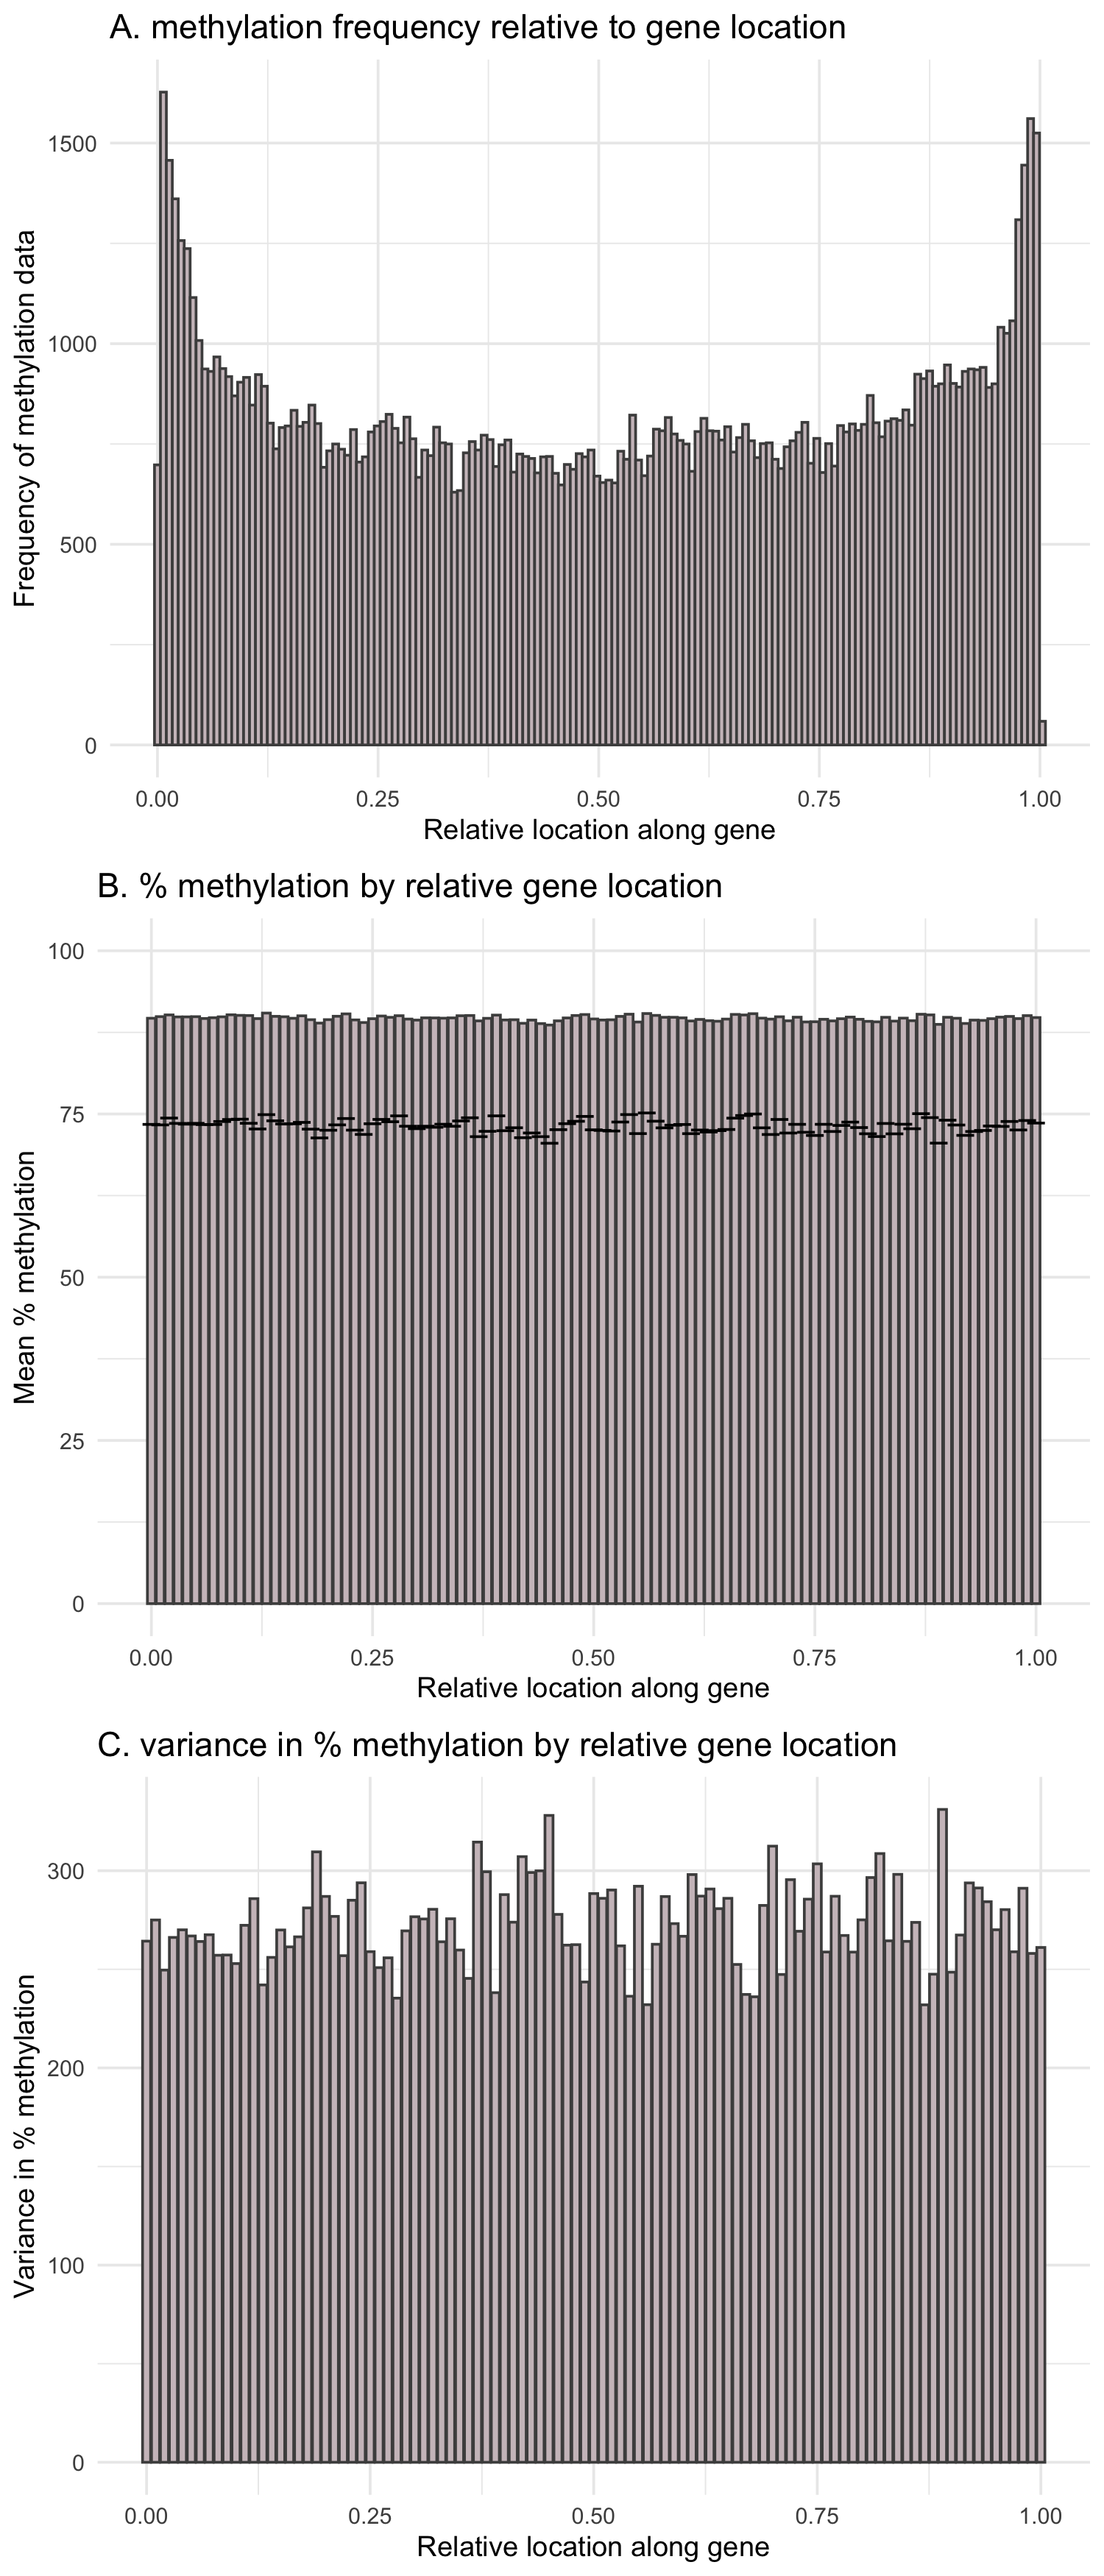
\includegraphics[width=0.6\textwidth,height=\textheight]{../supplemental-files/Supp-03.png}
\caption{\textbf{Supplemental Figure 3:} Gene body methylation patterns.
A) relative location of methylation within gene bodies in \emph{Ostrea
lurida}. For this analysis methylated loci were designated as those with
\textgreater50\% methylation when averaged across all MBD18 samples, B)
percent methylation across a gene body averaged across all MBD18
samples, and C) variation in percent methylation across a gene body,
across all MBD18 samples.}
\end{figure}

****:

\begin{center}\rule{0.5\linewidth}{0.5pt}\end{center}

\textbf{Supplemental Table 1}: Biological functions that are enriched in
the \emph{Ostrea lurida} genome. Also available in .csv format:
\url{https://github.com/sr320/paper-oly-mbdbs-gen/blob/master/analyses/methylation-characteristics/methylated-loci-enriched-BP.csv}

\begin{longtable}[]{@{}lllll@{}}
\toprule
\begin{minipage}[b]{0.17\columnwidth}\raggedright
GO Term\strut
\end{minipage} & \begin{minipage}[b]{0.17\columnwidth}\raggedright
Biological Process\strut
\end{minipage} & \begin{minipage}[b]{0.17\columnwidth}\raggedright
PValue\strut
\end{minipage} & \begin{minipage}[b]{0.17\columnwidth}\raggedright
FDR\strut
\end{minipage} & \begin{minipage}[b]{0.17\columnwidth}\raggedright
GO slim\strut
\end{minipage}\tabularnewline
\midrule
\endhead
\begin{minipage}[t]{0.17\columnwidth}\raggedright
\url{GO:0007067}\strut
\end{minipage} & \begin{minipage}[t]{0.17\columnwidth}\raggedright
mitotic nuclear division\strut
\end{minipage} & \begin{minipage}[t]{0.17\columnwidth}\raggedright
0\strut
\end{minipage} & \begin{minipage}[t]{0.17\columnwidth}\raggedright
0.37\strut
\end{minipage} & \begin{minipage}[t]{0.17\columnwidth}\raggedright
cell cycle and proliferation\strut
\end{minipage}\tabularnewline
\begin{minipage}[t]{0.17\columnwidth}\raggedright
\url{GO:0007049}\strut
\end{minipage} & \begin{minipage}[t]{0.17\columnwidth}\raggedright
cell cycle\strut
\end{minipage} & \begin{minipage}[t]{0.17\columnwidth}\raggedright
0\strut
\end{minipage} & \begin{minipage}[t]{0.17\columnwidth}\raggedright
0.66\strut
\end{minipage} & \begin{minipage}[t]{0.17\columnwidth}\raggedright
cell cycle and proliferation\strut
\end{minipage}\tabularnewline
\begin{minipage}[t]{0.17\columnwidth}\raggedright
\url{GO:0051321}\strut
\end{minipage} & \begin{minipage}[t]{0.17\columnwidth}\raggedright
meiotic cell cycle\strut
\end{minipage} & \begin{minipage}[t]{0.17\columnwidth}\raggedright
0.05\strut
\end{minipage} & \begin{minipage}[t]{0.17\columnwidth}\raggedright
1\strut
\end{minipage} & \begin{minipage}[t]{0.17\columnwidth}\raggedright
cell cycle and proliferation\strut
\end{minipage}\tabularnewline
\begin{minipage}[t]{0.17\columnwidth}\raggedright
\url{GO:0000082}\strut
\end{minipage} & \begin{minipage}[t]{0.17\columnwidth}\raggedright
G1/S transition of mitotic cell cycle\strut
\end{minipage} & \begin{minipage}[t]{0.17\columnwidth}\raggedright
0.07\strut
\end{minipage} & \begin{minipage}[t]{0.17\columnwidth}\raggedright
1\strut
\end{minipage} & \begin{minipage}[t]{0.17\columnwidth}\raggedright
cell cycle and proliferation\strut
\end{minipage}\tabularnewline
\begin{minipage}[t]{0.17\columnwidth}\raggedright
\url{GO:0000086}\strut
\end{minipage} & \begin{minipage}[t]{0.17\columnwidth}\raggedright
G2/M transition of mitotic cell cycle\strut
\end{minipage} & \begin{minipage}[t]{0.17\columnwidth}\raggedright
0.09\strut
\end{minipage} & \begin{minipage}[t]{0.17\columnwidth}\raggedright
1\strut
\end{minipage} & \begin{minipage}[t]{0.17\columnwidth}\raggedright
cell cycle and proliferation\strut
\end{minipage}\tabularnewline
\begin{minipage}[t]{0.17\columnwidth}\raggedright
\url{GO:0007067}\strut
\end{minipage} & \begin{minipage}[t]{0.17\columnwidth}\raggedright
mitotic nuclear division\strut
\end{minipage} & \begin{minipage}[t]{0.17\columnwidth}\raggedright
0\strut
\end{minipage} & \begin{minipage}[t]{0.17\columnwidth}\raggedright
0.37\strut
\end{minipage} & \begin{minipage}[t]{0.17\columnwidth}\raggedright
cell organization and biogenesis\strut
\end{minipage}\tabularnewline
\begin{minipage}[t]{0.17\columnwidth}\raggedright
\url{GO:0016569}\strut
\end{minipage} & \begin{minipage}[t]{0.17\columnwidth}\raggedright
covalent chromatin modification\strut
\end{minipage} & \begin{minipage}[t]{0.17\columnwidth}\raggedright
0.01\strut
\end{minipage} & \begin{minipage}[t]{0.17\columnwidth}\raggedright
1\strut
\end{minipage} & \begin{minipage}[t]{0.17\columnwidth}\raggedright
cell organization and biogenesis\strut
\end{minipage}\tabularnewline
\begin{minipage}[t]{0.17\columnwidth}\raggedright
\url{GO:0060271}\strut
\end{minipage} & \begin{minipage}[t]{0.17\columnwidth}\raggedright
cilium morphogenesis\strut
\end{minipage} & \begin{minipage}[t]{0.17\columnwidth}\raggedright
0.01\strut
\end{minipage} & \begin{minipage}[t]{0.17\columnwidth}\raggedright
1\strut
\end{minipage} & \begin{minipage}[t]{0.17\columnwidth}\raggedright
cell organization and biogenesis\strut
\end{minipage}\tabularnewline
\begin{minipage}[t]{0.17\columnwidth}\raggedright
\url{GO:0042384}\strut
\end{minipage} & \begin{minipage}[t]{0.17\columnwidth}\raggedright
cilium assembly\strut
\end{minipage} & \begin{minipage}[t]{0.17\columnwidth}\raggedright
0.01\strut
\end{minipage} & \begin{minipage}[t]{0.17\columnwidth}\raggedright
1\strut
\end{minipage} & \begin{minipage}[t]{0.17\columnwidth}\raggedright
cell organization and biogenesis\strut
\end{minipage}\tabularnewline
\begin{minipage}[t]{0.17\columnwidth}\raggedright
\url{GO:0007030}\strut
\end{minipage} & \begin{minipage}[t]{0.17\columnwidth}\raggedright
Golgi organization\strut
\end{minipage} & \begin{minipage}[t]{0.17\columnwidth}\raggedright
0.02\strut
\end{minipage} & \begin{minipage}[t]{0.17\columnwidth}\raggedright
1\strut
\end{minipage} & \begin{minipage}[t]{0.17\columnwidth}\raggedright
cell organization and biogenesis\strut
\end{minipage}\tabularnewline
\begin{minipage}[t]{0.17\columnwidth}\raggedright
\url{GO:0030030}\strut
\end{minipage} & \begin{minipage}[t]{0.17\columnwidth}\raggedright
cell projection organization\strut
\end{minipage} & \begin{minipage}[t]{0.17\columnwidth}\raggedright
0.05\strut
\end{minipage} & \begin{minipage}[t]{0.17\columnwidth}\raggedright
1\strut
\end{minipage} & \begin{minipage}[t]{0.17\columnwidth}\raggedright
cell organization and biogenesis\strut
\end{minipage}\tabularnewline
\begin{minipage}[t]{0.17\columnwidth}\raggedright
\url{GO:0007005}\strut
\end{minipage} & \begin{minipage}[t]{0.17\columnwidth}\raggedright
mitochondrion organization\strut
\end{minipage} & \begin{minipage}[t]{0.17\columnwidth}\raggedright
0.05\strut
\end{minipage} & \begin{minipage}[t]{0.17\columnwidth}\raggedright
1\strut
\end{minipage} & \begin{minipage}[t]{0.17\columnwidth}\raggedright
cell organization and biogenesis\strut
\end{minipage}\tabularnewline
\begin{minipage}[t]{0.17\columnwidth}\raggedright
\url{GO:0001822}\strut
\end{minipage} & \begin{minipage}[t]{0.17\columnwidth}\raggedright
kidney development\strut
\end{minipage} & \begin{minipage}[t]{0.17\columnwidth}\raggedright
0.02\strut
\end{minipage} & \begin{minipage}[t]{0.17\columnwidth}\raggedright
1\strut
\end{minipage} & \begin{minipage}[t]{0.17\columnwidth}\raggedright
developmental processes\strut
\end{minipage}\tabularnewline
\begin{minipage}[t]{0.17\columnwidth}\raggedright
\url{GO:0001843}\strut
\end{minipage} & \begin{minipage}[t]{0.17\columnwidth}\raggedright
neural tube closure\strut
\end{minipage} & \begin{minipage}[t]{0.17\columnwidth}\raggedright
0.07\strut
\end{minipage} & \begin{minipage}[t]{0.17\columnwidth}\raggedright
1\strut
\end{minipage} & \begin{minipage}[t]{0.17\columnwidth}\raggedright
developmental processes\strut
\end{minipage}\tabularnewline
\begin{minipage}[t]{0.17\columnwidth}\raggedright
\url{GO:0006281}\strut
\end{minipage} & \begin{minipage}[t]{0.17\columnwidth}\raggedright
DNA repair\strut
\end{minipage} & \begin{minipage}[t]{0.17\columnwidth}\raggedright
0\strut
\end{minipage} & \begin{minipage}[t]{0.17\columnwidth}\raggedright
0.08\strut
\end{minipage} & \begin{minipage}[t]{0.17\columnwidth}\raggedright
DNA metabolism\strut
\end{minipage}\tabularnewline
\begin{minipage}[t]{0.17\columnwidth}\raggedright
\url{GO:0006260}\strut
\end{minipage} & \begin{minipage}[t]{0.17\columnwidth}\raggedright
DNA replication\strut
\end{minipage} & \begin{minipage}[t]{0.17\columnwidth}\raggedright
0\strut
\end{minipage} & \begin{minipage}[t]{0.17\columnwidth}\raggedright
0.37\strut
\end{minipage} & \begin{minipage}[t]{0.17\columnwidth}\raggedright
DNA metabolism\strut
\end{minipage}\tabularnewline
\begin{minipage}[t]{0.17\columnwidth}\raggedright
\url{GO:0006310}\strut
\end{minipage} & \begin{minipage}[t]{0.17\columnwidth}\raggedright
DNA recombination\strut
\end{minipage} & \begin{minipage}[t]{0.17\columnwidth}\raggedright
0.04\strut
\end{minipage} & \begin{minipage}[t]{0.17\columnwidth}\raggedright
1\strut
\end{minipage} & \begin{minipage}[t]{0.17\columnwidth}\raggedright
DNA metabolism\strut
\end{minipage}\tabularnewline
\begin{minipage}[t]{0.17\columnwidth}\raggedright
\url{GO:0006302}\strut
\end{minipage} & \begin{minipage}[t]{0.17\columnwidth}\raggedright
double-strand break repair\strut
\end{minipage} & \begin{minipage}[t]{0.17\columnwidth}\raggedright
0.08\strut
\end{minipage} & \begin{minipage}[t]{0.17\columnwidth}\raggedright
1\strut
\end{minipage} & \begin{minipage}[t]{0.17\columnwidth}\raggedright
DNA metabolism\strut
\end{minipage}\tabularnewline
\begin{minipage}[t]{0.17\columnwidth}\raggedright
\url{GO:0006284}\strut
\end{minipage} & \begin{minipage}[t]{0.17\columnwidth}\raggedright
base-excision repair\strut
\end{minipage} & \begin{minipage}[t]{0.17\columnwidth}\raggedright
0.09\strut
\end{minipage} & \begin{minipage}[t]{0.17\columnwidth}\raggedright
1\strut
\end{minipage} & \begin{minipage}[t]{0.17\columnwidth}\raggedright
DNA metabolism\strut
\end{minipage}\tabularnewline
\begin{minipage}[t]{0.17\columnwidth}\raggedright
\url{GO:0051301}\strut
\end{minipage} & \begin{minipage}[t]{0.17\columnwidth}\raggedright
cell division\strut
\end{minipage} & \begin{minipage}[t]{0.17\columnwidth}\raggedright
0\strut
\end{minipage} & \begin{minipage}[t]{0.17\columnwidth}\raggedright
0.12\strut
\end{minipage} & \begin{minipage}[t]{0.17\columnwidth}\raggedright
other biological processes\strut
\end{minipage}\tabularnewline
\begin{minipage}[t]{0.17\columnwidth}\raggedright
\url{GO:0007018}\strut
\end{minipage} & \begin{minipage}[t]{0.17\columnwidth}\raggedright
microtubule-based movement\strut
\end{minipage} & \begin{minipage}[t]{0.17\columnwidth}\raggedright
0.02\strut
\end{minipage} & \begin{minipage}[t]{0.17\columnwidth}\raggedright
1\strut
\end{minipage} & \begin{minipage}[t]{0.17\columnwidth}\raggedright
other biological processes\strut
\end{minipage}\tabularnewline
\begin{minipage}[t]{0.17\columnwidth}\raggedright
\url{GO:0042254}\strut
\end{minipage} & \begin{minipage}[t]{0.17\columnwidth}\raggedright
ribosome biogenesis\strut
\end{minipage} & \begin{minipage}[t]{0.17\columnwidth}\raggedright
0.05\strut
\end{minipage} & \begin{minipage}[t]{0.17\columnwidth}\raggedright
1\strut
\end{minipage} & \begin{minipage}[t]{0.17\columnwidth}\raggedright
other biological processes\strut
\end{minipage}\tabularnewline
\begin{minipage}[t]{0.17\columnwidth}\raggedright
\url{GO:0016032}\strut
\end{minipage} & \begin{minipage}[t]{0.17\columnwidth}\raggedright
viral process\strut
\end{minipage} & \begin{minipage}[t]{0.17\columnwidth}\raggedright
0.05\strut
\end{minipage} & \begin{minipage}[t]{0.17\columnwidth}\raggedright
1\strut
\end{minipage} & \begin{minipage}[t]{0.17\columnwidth}\raggedright
other biological processes\strut
\end{minipage}\tabularnewline
\begin{minipage}[t]{0.17\columnwidth}\raggedright
\url{GO:0043547}\strut
\end{minipage} & \begin{minipage}[t]{0.17\columnwidth}\raggedright
positive regulation of GTPase activity\strut
\end{minipage} & \begin{minipage}[t]{0.17\columnwidth}\raggedright
0.05\strut
\end{minipage} & \begin{minipage}[t]{0.17\columnwidth}\raggedright
1\strut
\end{minipage} & \begin{minipage}[t]{0.17\columnwidth}\raggedright
other biological processes\strut
\end{minipage}\tabularnewline
\begin{minipage}[t]{0.17\columnwidth}\raggedright
\url{GO:0000910}\strut
\end{minipage} & \begin{minipage}[t]{0.17\columnwidth}\raggedright
cytokinesis\strut
\end{minipage} & \begin{minipage}[t]{0.17\columnwidth}\raggedright
0.06\strut
\end{minipage} & \begin{minipage}[t]{0.17\columnwidth}\raggedright
1\strut
\end{minipage} & \begin{minipage}[t]{0.17\columnwidth}\raggedright
other biological processes\strut
\end{minipage}\tabularnewline
\begin{minipage}[t]{0.17\columnwidth}\raggedright
\url{GO:0032092}\strut
\end{minipage} & \begin{minipage}[t]{0.17\columnwidth}\raggedright
positive regulation of protein binding\strut
\end{minipage} & \begin{minipage}[t]{0.17\columnwidth}\raggedright
0.08\strut
\end{minipage} & \begin{minipage}[t]{0.17\columnwidth}\raggedright
1\strut
\end{minipage} & \begin{minipage}[t]{0.17\columnwidth}\raggedright
other biological processes\strut
\end{minipage}\tabularnewline
\begin{minipage}[t]{0.17\columnwidth}\raggedright
\url{GO:0008104}\strut
\end{minipage} & \begin{minipage}[t]{0.17\columnwidth}\raggedright
protein localization\strut
\end{minipage} & \begin{minipage}[t]{0.17\columnwidth}\raggedright
0.09\strut
\end{minipage} & \begin{minipage}[t]{0.17\columnwidth}\raggedright
1\strut
\end{minipage} & \begin{minipage}[t]{0.17\columnwidth}\raggedright
other biological processes\strut
\end{minipage}\tabularnewline
\begin{minipage}[t]{0.17\columnwidth}\raggedright
\url{GO:0031047}\strut
\end{minipage} & \begin{minipage}[t]{0.17\columnwidth}\raggedright
gene silencing by RNA\strut
\end{minipage} & \begin{minipage}[t]{0.17\columnwidth}\raggedright
0.01\strut
\end{minipage} & \begin{minipage}[t]{0.17\columnwidth}\raggedright
1\strut
\end{minipage} & \begin{minipage}[t]{0.17\columnwidth}\raggedright
other metabolic processes\strut
\end{minipage}\tabularnewline
\begin{minipage}[t]{0.17\columnwidth}\raggedright
\url{GO:0006511}\strut
\end{minipage} & \begin{minipage}[t]{0.17\columnwidth}\raggedright
ubiquitin-dependent protein catabolic process\strut
\end{minipage} & \begin{minipage}[t]{0.17\columnwidth}\raggedright
0\strut
\end{minipage} & \begin{minipage}[t]{0.17\columnwidth}\raggedright
0.12\strut
\end{minipage} & \begin{minipage}[t]{0.17\columnwidth}\raggedright
protein metabolism\strut
\end{minipage}\tabularnewline
\begin{minipage}[t]{0.17\columnwidth}\raggedright
\url{GO:0006412}\strut
\end{minipage} & \begin{minipage}[t]{0.17\columnwidth}\raggedright
translation\strut
\end{minipage} & \begin{minipage}[t]{0.17\columnwidth}\raggedright
0\strut
\end{minipage} & \begin{minipage}[t]{0.17\columnwidth}\raggedright
0.37\strut
\end{minipage} & \begin{minipage}[t]{0.17\columnwidth}\raggedright
protein metabolism\strut
\end{minipage}\tabularnewline
\begin{minipage}[t]{0.17\columnwidth}\raggedright
\url{GO:0050821}\strut
\end{minipage} & \begin{minipage}[t]{0.17\columnwidth}\raggedright
protein stabilization\strut
\end{minipage} & \begin{minipage}[t]{0.17\columnwidth}\raggedright
0.01\strut
\end{minipage} & \begin{minipage}[t]{0.17\columnwidth}\raggedright
1\strut
\end{minipage} & \begin{minipage}[t]{0.17\columnwidth}\raggedright
protein metabolism\strut
\end{minipage}\tabularnewline
\begin{minipage}[t]{0.17\columnwidth}\raggedright
\url{GO:0006468}\strut
\end{minipage} & \begin{minipage}[t]{0.17\columnwidth}\raggedright
protein phosphorylation\strut
\end{minipage} & \begin{minipage}[t]{0.17\columnwidth}\raggedright
0.01\strut
\end{minipage} & \begin{minipage}[t]{0.17\columnwidth}\raggedright
1\strut
\end{minipage} & \begin{minipage}[t]{0.17\columnwidth}\raggedright
protein metabolism\strut
\end{minipage}\tabularnewline
\begin{minipage}[t]{0.17\columnwidth}\raggedright
\url{GO:0006413}\strut
\end{minipage} & \begin{minipage}[t]{0.17\columnwidth}\raggedright
translational initiation\strut
\end{minipage} & \begin{minipage}[t]{0.17\columnwidth}\raggedright
0.03\strut
\end{minipage} & \begin{minipage}[t]{0.17\columnwidth}\raggedright
1\strut
\end{minipage} & \begin{minipage}[t]{0.17\columnwidth}\raggedright
protein metabolism\strut
\end{minipage}\tabularnewline
\begin{minipage}[t]{0.17\columnwidth}\raggedright
\url{GO:0000209}\strut
\end{minipage} & \begin{minipage}[t]{0.17\columnwidth}\raggedright
protein polyubiquitination\strut
\end{minipage} & \begin{minipage}[t]{0.17\columnwidth}\raggedright
0.06\strut
\end{minipage} & \begin{minipage}[t]{0.17\columnwidth}\raggedright
1\strut
\end{minipage} & \begin{minipage}[t]{0.17\columnwidth}\raggedright
protein metabolism\strut
\end{minipage}\tabularnewline
\begin{minipage}[t]{0.17\columnwidth}\raggedright
\url{GO:0042787}\strut
\end{minipage} & \begin{minipage}[t]{0.17\columnwidth}\raggedright
protein ubiquitination involved in ubiquitin-dependent protein catabolic
process\strut
\end{minipage} & \begin{minipage}[t]{0.17\columnwidth}\raggedright
0.08\strut
\end{minipage} & \begin{minipage}[t]{0.17\columnwidth}\raggedright
1\strut
\end{minipage} & \begin{minipage}[t]{0.17\columnwidth}\raggedright
protein metabolism\strut
\end{minipage}\tabularnewline
\begin{minipage}[t]{0.17\columnwidth}\raggedright
\url{GO:0016567}\strut
\end{minipage} & \begin{minipage}[t]{0.17\columnwidth}\raggedright
protein ubiquitination\strut
\end{minipage} & \begin{minipage}[t]{0.17\columnwidth}\raggedright
0.09\strut
\end{minipage} & \begin{minipage}[t]{0.17\columnwidth}\raggedright
1\strut
\end{minipage} & \begin{minipage}[t]{0.17\columnwidth}\raggedright
protein metabolism\strut
\end{minipage}\tabularnewline
\begin{minipage}[t]{0.17\columnwidth}\raggedright
\url{GO:0000398}\strut
\end{minipage} & \begin{minipage}[t]{0.17\columnwidth}\raggedright
mRNA splicing, via spliceosome\strut
\end{minipage} & \begin{minipage}[t]{0.17\columnwidth}\raggedright
0\strut
\end{minipage} & \begin{minipage}[t]{0.17\columnwidth}\raggedright
0.53\strut
\end{minipage} & \begin{minipage}[t]{0.17\columnwidth}\raggedright
RNA metabolism\strut
\end{minipage}\tabularnewline
\begin{minipage}[t]{0.17\columnwidth}\raggedright
\url{GO:0006397}\strut
\end{minipage} & \begin{minipage}[t]{0.17\columnwidth}\raggedright
mRNA processing\strut
\end{minipage} & \begin{minipage}[t]{0.17\columnwidth}\raggedright
0\strut
\end{minipage} & \begin{minipage}[t]{0.17\columnwidth}\raggedright
1\strut
\end{minipage} & \begin{minipage}[t]{0.17\columnwidth}\raggedright
RNA metabolism\strut
\end{minipage}\tabularnewline
\begin{minipage}[t]{0.17\columnwidth}\raggedright
\url{GO:0006364}\strut
\end{minipage} & \begin{minipage}[t]{0.17\columnwidth}\raggedright
rRNA processing\strut
\end{minipage} & \begin{minipage}[t]{0.17\columnwidth}\raggedright
0.01\strut
\end{minipage} & \begin{minipage}[t]{0.17\columnwidth}\raggedright
1\strut
\end{minipage} & \begin{minipage}[t]{0.17\columnwidth}\raggedright
RNA metabolism\strut
\end{minipage}\tabularnewline
\begin{minipage}[t]{0.17\columnwidth}\raggedright
\url{GO:0006396}\strut
\end{minipage} & \begin{minipage}[t]{0.17\columnwidth}\raggedright
RNA processing\strut
\end{minipage} & \begin{minipage}[t]{0.17\columnwidth}\raggedright
0.01\strut
\end{minipage} & \begin{minipage}[t]{0.17\columnwidth}\raggedright
1\strut
\end{minipage} & \begin{minipage}[t]{0.17\columnwidth}\raggedright
RNA metabolism\strut
\end{minipage}\tabularnewline
\begin{minipage}[t]{0.17\columnwidth}\raggedright
\url{GO:0008380}\strut
\end{minipage} & \begin{minipage}[t]{0.17\columnwidth}\raggedright
RNA splicing\strut
\end{minipage} & \begin{minipage}[t]{0.17\columnwidth}\raggedright
0.02\strut
\end{minipage} & \begin{minipage}[t]{0.17\columnwidth}\raggedright
1\strut
\end{minipage} & \begin{minipage}[t]{0.17\columnwidth}\raggedright
RNA metabolism\strut
\end{minipage}\tabularnewline
\begin{minipage}[t]{0.17\columnwidth}\raggedright
\url{GO:0006366}\strut
\end{minipage} & \begin{minipage}[t]{0.17\columnwidth}\raggedright
transcription from RNA polymerase II promoter\strut
\end{minipage} & \begin{minipage}[t]{0.17\columnwidth}\raggedright
0.05\strut
\end{minipage} & \begin{minipage}[t]{0.17\columnwidth}\raggedright
1\strut
\end{minipage} & \begin{minipage}[t]{0.17\columnwidth}\raggedright
RNA metabolism\strut
\end{minipage}\tabularnewline
\begin{minipage}[t]{0.17\columnwidth}\raggedright
\url{GO:0008033}\strut
\end{minipage} & \begin{minipage}[t]{0.17\columnwidth}\raggedright
tRNA processing\strut
\end{minipage} & \begin{minipage}[t]{0.17\columnwidth}\raggedright
0.06\strut
\end{minipage} & \begin{minipage}[t]{0.17\columnwidth}\raggedright
1\strut
\end{minipage} & \begin{minipage}[t]{0.17\columnwidth}\raggedright
RNA metabolism\strut
\end{minipage}\tabularnewline
\begin{minipage}[t]{0.17\columnwidth}\raggedright
\url{GO:0006355}\strut
\end{minipage} & \begin{minipage}[t]{0.17\columnwidth}\raggedright
regulation of transcription, DNA-templated\strut
\end{minipage} & \begin{minipage}[t]{0.17\columnwidth}\raggedright
0.09\strut
\end{minipage} & \begin{minipage}[t]{0.17\columnwidth}\raggedright
1\strut
\end{minipage} & \begin{minipage}[t]{0.17\columnwidth}\raggedright
RNA metabolism\strut
\end{minipage}\tabularnewline
\begin{minipage}[t]{0.17\columnwidth}\raggedright
\url{GO:0006974}\strut
\end{minipage} & \begin{minipage}[t]{0.17\columnwidth}\raggedright
cellular response to DNA damage stimulus\strut
\end{minipage} & \begin{minipage}[t]{0.17\columnwidth}\raggedright
0\strut
\end{minipage} & \begin{minipage}[t]{0.17\columnwidth}\raggedright
0.05\strut
\end{minipage} & \begin{minipage}[t]{0.17\columnwidth}\raggedright
stress response\strut
\end{minipage}\tabularnewline
\begin{minipage}[t]{0.17\columnwidth}\raggedright
\url{GO:0006281}\strut
\end{minipage} & \begin{minipage}[t]{0.17\columnwidth}\raggedright
DNA repair\strut
\end{minipage} & \begin{minipage}[t]{0.17\columnwidth}\raggedright
0\strut
\end{minipage} & \begin{minipage}[t]{0.17\columnwidth}\raggedright
0.08\strut
\end{minipage} & \begin{minipage}[t]{0.17\columnwidth}\raggedright
stress response\strut
\end{minipage}\tabularnewline
\begin{minipage}[t]{0.17\columnwidth}\raggedright
\url{GO:0006302}\strut
\end{minipage} & \begin{minipage}[t]{0.17\columnwidth}\raggedright
double-strand break repair\strut
\end{minipage} & \begin{minipage}[t]{0.17\columnwidth}\raggedright
0.08\strut
\end{minipage} & \begin{minipage}[t]{0.17\columnwidth}\raggedright
1\strut
\end{minipage} & \begin{minipage}[t]{0.17\columnwidth}\raggedright
stress response\strut
\end{minipage}\tabularnewline
\begin{minipage}[t]{0.17\columnwidth}\raggedright
\url{GO:0006284}\strut
\end{minipage} & \begin{minipage}[t]{0.17\columnwidth}\raggedright
base-excision repair\strut
\end{minipage} & \begin{minipage}[t]{0.17\columnwidth}\raggedright
0.09\strut
\end{minipage} & \begin{minipage}[t]{0.17\columnwidth}\raggedright
1\strut
\end{minipage} & \begin{minipage}[t]{0.17\columnwidth}\raggedright
stress response\strut
\end{minipage}\tabularnewline
\begin{minipage}[t]{0.17\columnwidth}\raggedright
\url{GO:0015031}\strut
\end{minipage} & \begin{minipage}[t]{0.17\columnwidth}\raggedright
protein transport\strut
\end{minipage} & \begin{minipage}[t]{0.17\columnwidth}\raggedright
0\strut
\end{minipage} & \begin{minipage}[t]{0.17\columnwidth}\raggedright
0.23\strut
\end{minipage} & \begin{minipage}[t]{0.17\columnwidth}\raggedright
transport\strut
\end{minipage}\tabularnewline
\begin{minipage}[t]{0.17\columnwidth}\raggedright
\url{GO:0006886}\strut
\end{minipage} & \begin{minipage}[t]{0.17\columnwidth}\raggedright
intracellular protein transport\strut
\end{minipage} & \begin{minipage}[t]{0.17\columnwidth}\raggedright
0\strut
\end{minipage} & \begin{minipage}[t]{0.17\columnwidth}\raggedright
0.81\strut
\end{minipage} & \begin{minipage}[t]{0.17\columnwidth}\raggedright
transport\strut
\end{minipage}\tabularnewline
\begin{minipage}[t]{0.17\columnwidth}\raggedright
\url{GO:0006888}\strut
\end{minipage} & \begin{minipage}[t]{0.17\columnwidth}\raggedright
ER to Golgi vesicle-mediated transport\strut
\end{minipage} & \begin{minipage}[t]{0.17\columnwidth}\raggedright
0\strut
\end{minipage} & \begin{minipage}[t]{0.17\columnwidth}\raggedright
0.96\strut
\end{minipage} & \begin{minipage}[t]{0.17\columnwidth}\raggedright
transport\strut
\end{minipage}\tabularnewline
\begin{minipage}[t]{0.17\columnwidth}\raggedright
\url{GO:0016192}\strut
\end{minipage} & \begin{minipage}[t]{0.17\columnwidth}\raggedright
vesicle-mediated transport\strut
\end{minipage} & \begin{minipage}[t]{0.17\columnwidth}\raggedright
0.02\strut
\end{minipage} & \begin{minipage}[t]{0.17\columnwidth}\raggedright
1\strut
\end{minipage} & \begin{minipage}[t]{0.17\columnwidth}\raggedright
transport\strut
\end{minipage}\tabularnewline
\begin{minipage}[t]{0.17\columnwidth}\raggedright
\url{GO:0006406}\strut
\end{minipage} & \begin{minipage}[t]{0.17\columnwidth}\raggedright
mRNA export from nucleus\strut
\end{minipage} & \begin{minipage}[t]{0.17\columnwidth}\raggedright
0.04\strut
\end{minipage} & \begin{minipage}[t]{0.17\columnwidth}\raggedright
1\strut
\end{minipage} & \begin{minipage}[t]{0.17\columnwidth}\raggedright
transport\strut
\end{minipage}\tabularnewline
\begin{minipage}[t]{0.17\columnwidth}\raggedright
\url{GO:0006606}\strut
\end{minipage} & \begin{minipage}[t]{0.17\columnwidth}\raggedright
protein import into nucleus\strut
\end{minipage} & \begin{minipage}[t]{0.17\columnwidth}\raggedright
0.09\strut
\end{minipage} & \begin{minipage}[t]{0.17\columnwidth}\raggedright
1\strut
\end{minipage} & \begin{minipage}[t]{0.17\columnwidth}\raggedright
transport\strut
\end{minipage}\tabularnewline
\begin{minipage}[t]{0.17\columnwidth}\raggedright
\url{GO:0042147}\strut
\end{minipage} & \begin{minipage}[t]{0.17\columnwidth}\raggedright
retrograde transport, endosome to Golgi\strut
\end{minipage} & \begin{minipage}[t]{0.17\columnwidth}\raggedright
0.1\strut
\end{minipage} & \begin{minipage}[t]{0.17\columnwidth}\raggedright
1\strut
\end{minipage} & \begin{minipage}[t]{0.17\columnwidth}\raggedright
transport\strut
\end{minipage}\tabularnewline
\begin{minipage}[t]{0.17\columnwidth}\raggedright
\url{GO:0098609}\strut
\end{minipage} & \begin{minipage}[t]{0.17\columnwidth}\raggedright
cell-cell adhesion\strut
\end{minipage} & \begin{minipage}[t]{0.17\columnwidth}\raggedright
0.04\strut
\end{minipage} & \begin{minipage}[t]{0.17\columnwidth}\raggedright
1\strut
\end{minipage} & \begin{minipage}[t]{0.17\columnwidth}\raggedright
NA\strut
\end{minipage}\tabularnewline
\begin{minipage}[t]{0.17\columnwidth}\raggedright
\url{GO:0070936}\strut
\end{minipage} & \begin{minipage}[t]{0.17\columnwidth}\raggedright
protein K48-linked ubiquitination\strut
\end{minipage} & \begin{minipage}[t]{0.17\columnwidth}\raggedright
0.07\strut
\end{minipage} & \begin{minipage}[t]{0.17\columnwidth}\raggedright
1\strut
\end{minipage} & \begin{minipage}[t]{0.17\columnwidth}\raggedright
NA\strut
\end{minipage}\tabularnewline
\begin{minipage}[t]{0.17\columnwidth}\raggedright
\url{GO:0003341}\strut
\end{minipage} & \begin{minipage}[t]{0.17\columnwidth}\raggedright
cilium movement\strut
\end{minipage} & \begin{minipage}[t]{0.17\columnwidth}\raggedright
0.07\strut
\end{minipage} & \begin{minipage}[t]{0.17\columnwidth}\raggedright
1\strut
\end{minipage} & \begin{minipage}[t]{0.17\columnwidth}\raggedright
NA\strut
\end{minipage}\tabularnewline
\bottomrule
\end{longtable}

\begin{center}\rule{0.5\linewidth}{0.5pt}\end{center}

\hypertarget{differential-methylation-analysis-among-populations}{%
\subsubsection{2. Differential methylation analysis among
populations}\label{differential-methylation-analysis-among-populations}}

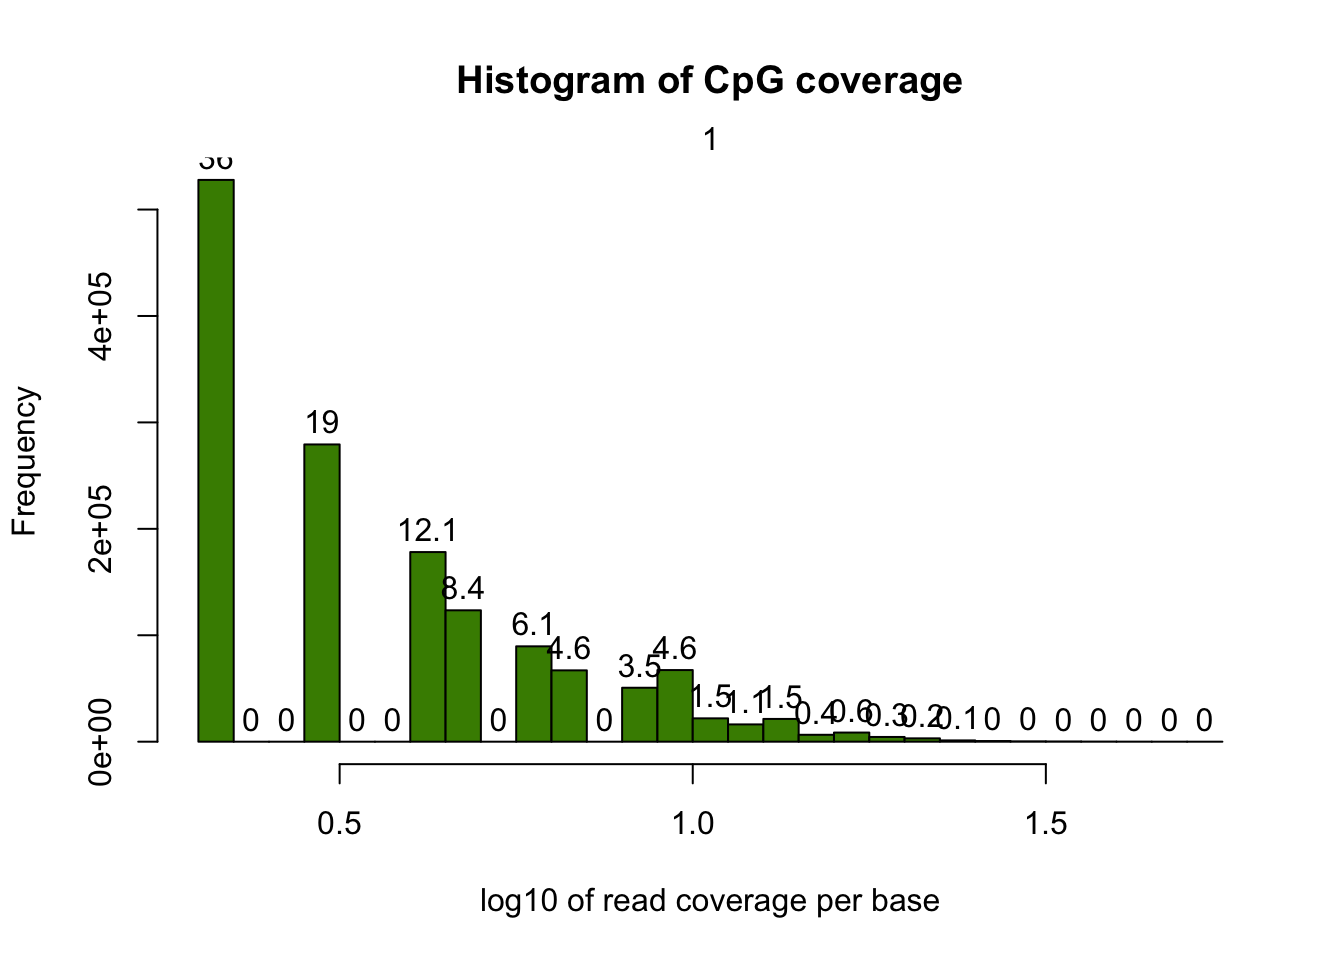
\includegraphics{Supplementary_files/figure-latex/unnamed-chunk-5-1.pdf}

\textbf{Supplemental Figure 4}: Heat map of loci that are differentially
methylated (DMLs) between the two populations.

\begin{center}\rule{0.5\linewidth}{0.5pt}\end{center}

\includegraphics{Supplementary_files/figure-latex/unnamed-chunk-6-1.pdf}

\textbf{Supplemental Figure 5}: PCA of methylation data using DMLs only

\begin{center}\rule{0.5\linewidth}{0.5pt}\end{center}

\includegraphics{Supplementary_files/figure-latex/unnamed-chunk-7-1.pdf}

\textbf{Supplemental Figure 6}: The \% difference between each
population's mean methylation for differentially methylated loci, which
highlights that both populations have a similar number of
hyper/hypo-methylated loci. Loci are sorted by \% methylation
difference.

\begin{center}\rule{0.5\linewidth}{0.5pt}\end{center}

\textbf{Supplemental Table 2}: GO terms and GO Slim terms of biological
functions enriched in DMGs \& DMLs. EASE scores shown. FDR for all terms
is 1.0. Also available in .csv format:
\url{https://github.com/sr320/paper-oly-mbdbs-gen/blob/master/analyses/DMG-DML-EnrichedBP.csv}

\begin{longtable}[]{@{}lllll@{}}
\toprule
\begin{minipage}[b]{0.17\columnwidth}\raggedright
Go Slim\strut
\end{minipage} & \begin{minipage}[b]{0.17\columnwidth}\raggedright
Term\strut
\end{minipage} & \begin{minipage}[b]{0.17\columnwidth}\raggedright
Function\strut
\end{minipage} & \begin{minipage}[b]{0.17\columnwidth}\raggedright
DMG\strut
\end{minipage} & \begin{minipage}[b]{0.17\columnwidth}\raggedright
DML\strut
\end{minipage}\tabularnewline
\midrule
\endhead
\begin{minipage}[t]{0.17\columnwidth}\raggedright
cell adhesion\strut
\end{minipage} & \begin{minipage}[t]{0.17\columnwidth}\raggedright
\url{GO:0007155}\strut
\end{minipage} & \begin{minipage}[t]{0.17\columnwidth}\raggedright
cell adhesion\strut
\end{minipage} & \begin{minipage}[t]{0.17\columnwidth}\raggedright
0.012\strut
\end{minipage} & \begin{minipage}[t]{0.17\columnwidth}\raggedright
\strut
\end{minipage}\tabularnewline
\begin{minipage}[t]{0.17\columnwidth}\raggedright
cell adhesion\strut
\end{minipage} & \begin{minipage}[t]{0.17\columnwidth}\raggedright
\url{GO:0007156}\strut
\end{minipage} & \begin{minipage}[t]{0.17\columnwidth}\raggedright
homophilic cell adhesion via plasma membrane adhesion molecules\strut
\end{minipage} & \begin{minipage}[t]{0.17\columnwidth}\raggedright
0.026\strut
\end{minipage} & \begin{minipage}[t]{0.17\columnwidth}\raggedright
0.00091\strut
\end{minipage}\tabularnewline
\begin{minipage}[t]{0.17\columnwidth}\raggedright
cell adhesion\strut
\end{minipage} & \begin{minipage}[t]{0.17\columnwidth}\raggedright
\url{GO:0016339}\strut
\end{minipage} & \begin{minipage}[t]{0.17\columnwidth}\raggedright
calcium-dependent cell-cell adhesion via plasma membrane cell adhesion
molecules\strut
\end{minipage} & \begin{minipage}[t]{0.17\columnwidth}\raggedright
\strut
\end{minipage} & \begin{minipage}[t]{0.17\columnwidth}\raggedright
0.083\strut
\end{minipage}\tabularnewline
\begin{minipage}[t]{0.17\columnwidth}\raggedright
cell organization and biogenesis\strut
\end{minipage} & \begin{minipage}[t]{0.17\columnwidth}\raggedright
\url{GO:0007015}\strut
\end{minipage} & \begin{minipage}[t]{0.17\columnwidth}\raggedright
actin filament organization\strut
\end{minipage} & \begin{minipage}[t]{0.17\columnwidth}\raggedright
0.014\strut
\end{minipage} & \begin{minipage}[t]{0.17\columnwidth}\raggedright
\strut
\end{minipage}\tabularnewline
\begin{minipage}[t]{0.17\columnwidth}\raggedright
cell organization and biogenesis\strut
\end{minipage} & \begin{minipage}[t]{0.17\columnwidth}\raggedright
\url{GO:0048675}\strut
\end{minipage} & \begin{minipage}[t]{0.17\columnwidth}\raggedright
axon extension\strut
\end{minipage} & \begin{minipage}[t]{0.17\columnwidth}\raggedright
0.047\strut
\end{minipage} & \begin{minipage}[t]{0.17\columnwidth}\raggedright
\strut
\end{minipage}\tabularnewline
\begin{minipage}[t]{0.17\columnwidth}\raggedright
cell organization and biogenesis\strut
\end{minipage} & \begin{minipage}[t]{0.17\columnwidth}\raggedright
\url{GO:0007411}\strut
\end{minipage} & \begin{minipage}[t]{0.17\columnwidth}\raggedright
axon guidance\strut
\end{minipage} & \begin{minipage}[t]{0.17\columnwidth}\raggedright
0.063\strut
\end{minipage} & \begin{minipage}[t]{0.17\columnwidth}\raggedright
\strut
\end{minipage}\tabularnewline
\begin{minipage}[t]{0.17\columnwidth}\raggedright
cell organization and biogenesis\strut
\end{minipage} & \begin{minipage}[t]{0.17\columnwidth}\raggedright
\url{GO:0000904}\strut
\end{minipage} & \begin{minipage}[t]{0.17\columnwidth}\raggedright
cell morphogenesis involved in differentiation\strut
\end{minipage} & \begin{minipage}[t]{0.17\columnwidth}\raggedright
0.095\strut
\end{minipage} & \begin{minipage}[t]{0.17\columnwidth}\raggedright
\strut
\end{minipage}\tabularnewline
\begin{minipage}[t]{0.17\columnwidth}\raggedright
cell organization and biogenesis\strut
\end{minipage} & \begin{minipage}[t]{0.17\columnwidth}\raggedright
\url{GO:0030198}\strut
\end{minipage} & \begin{minipage}[t]{0.17\columnwidth}\raggedright
extracellular matrix organization\strut
\end{minipage} & \begin{minipage}[t]{0.17\columnwidth}\raggedright
0.033\strut
\end{minipage} & \begin{minipage}[t]{0.17\columnwidth}\raggedright
\strut
\end{minipage}\tabularnewline
\begin{minipage}[t]{0.17\columnwidth}\raggedright
cell organization and biogenesis\strut
\end{minipage} & \begin{minipage}[t]{0.17\columnwidth}\raggedright
\url{GO:0032836}\strut
\end{minipage} & \begin{minipage}[t]{0.17\columnwidth}\raggedright
glomerular basement membrane development\strut
\end{minipage} & \begin{minipage}[t]{0.17\columnwidth}\raggedright
0.046\strut
\end{minipage} & \begin{minipage}[t]{0.17\columnwidth}\raggedright
\strut
\end{minipage}\tabularnewline
\begin{minipage}[t]{0.17\columnwidth}\raggedright
cell organization and biogenesis\strut
\end{minipage} & \begin{minipage}[t]{0.17\columnwidth}\raggedright
\url{GO:0007040}\strut
\end{minipage} & \begin{minipage}[t]{0.17\columnwidth}\raggedright
lysosome organization\strut
\end{minipage} & \begin{minipage}[t]{0.17\columnwidth}\raggedright
0.047\strut
\end{minipage} & \begin{minipage}[t]{0.17\columnwidth}\raggedright
\strut
\end{minipage}\tabularnewline
\begin{minipage}[t]{0.17\columnwidth}\raggedright
cell organization and biogenesis\strut
\end{minipage} & \begin{minipage}[t]{0.17\columnwidth}\raggedright
\url{GO:0031023}\strut
\end{minipage} & \begin{minipage}[t]{0.17\columnwidth}\raggedright
microtubule organizing center organization\strut
\end{minipage} & \begin{minipage}[t]{0.17\columnwidth}\raggedright
0.095\strut
\end{minipage} & \begin{minipage}[t]{0.17\columnwidth}\raggedright
\strut
\end{minipage}\tabularnewline
\begin{minipage}[t]{0.17\columnwidth}\raggedright
cell organization and biogenesis\strut
\end{minipage} & \begin{minipage}[t]{0.17\columnwidth}\raggedright
\url{GO:0051259}\strut
\end{minipage} & \begin{minipage}[t]{0.17\columnwidth}\raggedright
protein oligomerization\strut
\end{minipage} & \begin{minipage}[t]{0.17\columnwidth}\raggedright
0.098\strut
\end{minipage} & \begin{minipage}[t]{0.17\columnwidth}\raggedright
\strut
\end{minipage}\tabularnewline
\begin{minipage}[t]{0.17\columnwidth}\raggedright
cell organization and biogenesis\strut
\end{minipage} & \begin{minipage}[t]{0.17\columnwidth}\raggedright
\url{GO:0048841}\strut
\end{minipage} & \begin{minipage}[t]{0.17\columnwidth}\raggedright
regulation of axon extension involved in axon guidance\strut
\end{minipage} & \begin{minipage}[t]{0.17\columnwidth}\raggedright
0.033\strut
\end{minipage} & \begin{minipage}[t]{0.17\columnwidth}\raggedright
\strut
\end{minipage}\tabularnewline
\begin{minipage}[t]{0.17\columnwidth}\raggedright
cell organization and biogenesis\strut
\end{minipage} & \begin{minipage}[t]{0.17\columnwidth}\raggedright
\url{GO:0045214}\strut
\end{minipage} & \begin{minipage}[t]{0.17\columnwidth}\raggedright
sarcomere organization\strut
\end{minipage} & \begin{minipage}[t]{0.17\columnwidth}\raggedright
0.069\strut
\end{minipage} & \begin{minipage}[t]{0.17\columnwidth}\raggedright
0.019\strut
\end{minipage}\tabularnewline
\begin{minipage}[t]{0.17\columnwidth}\raggedright
cell organization and biogenesis\strut
\end{minipage} & \begin{minipage}[t]{0.17\columnwidth}\raggedright
\url{GO:0055003}\strut
\end{minipage} & \begin{minipage}[t]{0.17\columnwidth}\raggedright
cardiac myofibril assembly\strut
\end{minipage} & \begin{minipage}[t]{0.17\columnwidth}\raggedright
\strut
\end{minipage} & \begin{minipage}[t]{0.17\columnwidth}\raggedright
0.082\strut
\end{minipage}\tabularnewline
\begin{minipage}[t]{0.17\columnwidth}\raggedright
cell organization and biogenesis\strut
\end{minipage} & \begin{minipage}[t]{0.17\columnwidth}\raggedright
\url{GO:0032438}\strut
\end{minipage} & \begin{minipage}[t]{0.17\columnwidth}\raggedright
melanosome organization\strut
\end{minipage} & \begin{minipage}[t]{0.17\columnwidth}\raggedright
\strut
\end{minipage} & \begin{minipage}[t]{0.17\columnwidth}\raggedright
0.021\strut
\end{minipage}\tabularnewline
\begin{minipage}[t]{0.17\columnwidth}\raggedright
cell organization and biogenesis\strut
\end{minipage} & \begin{minipage}[t]{0.17\columnwidth}\raggedright
\url{GO:0045332}\strut
\end{minipage} & \begin{minipage}[t]{0.17\columnwidth}\raggedright
phospholipid translocation\strut
\end{minipage} & \begin{minipage}[t]{0.17\columnwidth}\raggedright
\strut
\end{minipage} & \begin{minipage}[t]{0.17\columnwidth}\raggedright
0.0058\strut
\end{minipage}\tabularnewline
\begin{minipage}[t]{0.17\columnwidth}\raggedright
death\strut
\end{minipage} & \begin{minipage}[t]{0.17\columnwidth}\raggedright
\url{GO:0008625}\strut
\end{minipage} & \begin{minipage}[t]{0.17\columnwidth}\raggedright
extrinsic apoptotic signaling pathway via death domain receptors\strut
\end{minipage} & \begin{minipage}[t]{0.17\columnwidth}\raggedright
0.095\strut
\end{minipage} & \begin{minipage}[t]{0.17\columnwidth}\raggedright
\strut
\end{minipage}\tabularnewline
\begin{minipage}[t]{0.17\columnwidth}\raggedright
developmental processes\strut
\end{minipage} & \begin{minipage}[t]{0.17\columnwidth}\raggedright
\url{GO:0048675}\strut
\end{minipage} & \begin{minipage}[t]{0.17\columnwidth}\raggedright
axon extension\strut
\end{minipage} & \begin{minipage}[t]{0.17\columnwidth}\raggedright
0.047\strut
\end{minipage} & \begin{minipage}[t]{0.17\columnwidth}\raggedright
\strut
\end{minipage}\tabularnewline
\begin{minipage}[t]{0.17\columnwidth}\raggedright
developmental processes\strut
\end{minipage} & \begin{minipage}[t]{0.17\columnwidth}\raggedright
\url{GO:0007411}\strut
\end{minipage} & \begin{minipage}[t]{0.17\columnwidth}\raggedright
axon guidance\strut
\end{minipage} & \begin{minipage}[t]{0.17\columnwidth}\raggedright
0.063\strut
\end{minipage} & \begin{minipage}[t]{0.17\columnwidth}\raggedright
\strut
\end{minipage}\tabularnewline
\begin{minipage}[t]{0.17\columnwidth}\raggedright
developmental processes\strut
\end{minipage} & \begin{minipage}[t]{0.17\columnwidth}\raggedright
\url{GO:0032836}\strut
\end{minipage} & \begin{minipage}[t]{0.17\columnwidth}\raggedright
glomerular basement membrane development\strut
\end{minipage} & \begin{minipage}[t]{0.17\columnwidth}\raggedright
0.046\strut
\end{minipage} & \begin{minipage}[t]{0.17\columnwidth}\raggedright
\strut
\end{minipage}\tabularnewline
\begin{minipage}[t]{0.17\columnwidth}\raggedright
developmental processes\strut
\end{minipage} & \begin{minipage}[t]{0.17\columnwidth}\raggedright
\url{GO:0048841}\strut
\end{minipage} & \begin{minipage}[t]{0.17\columnwidth}\raggedright
regulation of axon extension involved in axon guidance\strut
\end{minipage} & \begin{minipage}[t]{0.17\columnwidth}\raggedright
0.033\strut
\end{minipage} & \begin{minipage}[t]{0.17\columnwidth}\raggedright
\strut
\end{minipage}\tabularnewline
\begin{minipage}[t]{0.17\columnwidth}\raggedright
developmental processes\strut
\end{minipage} & \begin{minipage}[t]{0.17\columnwidth}\raggedright
\url{GO:0045214}\strut
\end{minipage} & \begin{minipage}[t]{0.17\columnwidth}\raggedright
sarcomere organization\strut
\end{minipage} & \begin{minipage}[t]{0.17\columnwidth}\raggedright
0.069\strut
\end{minipage} & \begin{minipage}[t]{0.17\columnwidth}\raggedright
0.019\strut
\end{minipage}\tabularnewline
\begin{minipage}[t]{0.17\columnwidth}\raggedright
developmental processes\strut
\end{minipage} & \begin{minipage}[t]{0.17\columnwidth}\raggedright
\url{GO:0007423}\strut
\end{minipage} & \begin{minipage}[t]{0.17\columnwidth}\raggedright
sensory organ development\strut
\end{minipage} & \begin{minipage}[t]{0.17\columnwidth}\raggedright
0.095\strut
\end{minipage} & \begin{minipage}[t]{0.17\columnwidth}\raggedright
\strut
\end{minipage}\tabularnewline
\begin{minipage}[t]{0.17\columnwidth}\raggedright
developmental processes\strut
\end{minipage} & \begin{minipage}[t]{0.17\columnwidth}\raggedright
\url{GO:0055003}\strut
\end{minipage} & \begin{minipage}[t]{0.17\columnwidth}\raggedright
cardiac myofibril assembly\strut
\end{minipage} & \begin{minipage}[t]{0.17\columnwidth}\raggedright
\strut
\end{minipage} & \begin{minipage}[t]{0.17\columnwidth}\raggedright
0.082\strut
\end{minipage}\tabularnewline
\begin{minipage}[t]{0.17\columnwidth}\raggedright
developmental processes\strut
\end{minipage} & \begin{minipage}[t]{0.17\columnwidth}\raggedright
\url{GO:0060429}\strut
\end{minipage} & \begin{minipage}[t]{0.17\columnwidth}\raggedright
epithelium development\strut
\end{minipage} & \begin{minipage}[t]{0.17\columnwidth}\raggedright
\strut
\end{minipage} & \begin{minipage}[t]{0.17\columnwidth}\raggedright
0.071\strut
\end{minipage}\tabularnewline
\begin{minipage}[t]{0.17\columnwidth}\raggedright
developmental processes\strut
\end{minipage} & \begin{minipage}[t]{0.17\columnwidth}\raggedright
\url{GO:0040027}\strut
\end{minipage} & \begin{minipage}[t]{0.17\columnwidth}\raggedright
negative regulation of vulval development\strut
\end{minipage} & \begin{minipage}[t]{0.17\columnwidth}\raggedright
\strut
\end{minipage} & \begin{minipage}[t]{0.17\columnwidth}\raggedright
0.082\strut
\end{minipage}\tabularnewline
\begin{minipage}[t]{0.17\columnwidth}\raggedright
developmental processes\strut
\end{minipage} & \begin{minipage}[t]{0.17\columnwidth}\raggedright
\url{GO:0021942}\strut
\end{minipage} & \begin{minipage}[t]{0.17\columnwidth}\raggedright
radial glia guided migration of Purkinje cell\strut
\end{minipage} & \begin{minipage}[t]{0.17\columnwidth}\raggedright
\strut
\end{minipage} & \begin{minipage}[t]{0.17\columnwidth}\raggedright
0.082\strut
\end{minipage}\tabularnewline
\begin{minipage}[t]{0.17\columnwidth}\raggedright
developmental processes\strut
\end{minipage} & \begin{minipage}[t]{0.17\columnwidth}\raggedright
\url{GO:0050767}\strut
\end{minipage} & \begin{minipage}[t]{0.17\columnwidth}\raggedright
regulation of neurogenesis\strut
\end{minipage} & \begin{minipage}[t]{0.17\columnwidth}\raggedright
\strut
\end{minipage} & \begin{minipage}[t]{0.17\columnwidth}\raggedright
0.0058\strut
\end{minipage}\tabularnewline
\begin{minipage}[t]{0.17\columnwidth}\raggedright
developmental processes\strut
\end{minipage} & \begin{minipage}[t]{0.17\columnwidth}\raggedright
\url{GO:0060438}\strut
\end{minipage} & \begin{minipage}[t]{0.17\columnwidth}\raggedright
trachea development\strut
\end{minipage} & \begin{minipage}[t]{0.17\columnwidth}\raggedright
\strut
\end{minipage} & \begin{minipage}[t]{0.17\columnwidth}\raggedright
0.082\strut
\end{minipage}\tabularnewline
\begin{minipage}[t]{0.17\columnwidth}\raggedright
developmental processes\strut
\end{minipage} & \begin{minipage}[t]{0.17\columnwidth}\raggedright
\url{GO:0001570}\strut
\end{minipage} & \begin{minipage}[t]{0.17\columnwidth}\raggedright
vasculogenesis\strut
\end{minipage} & \begin{minipage}[t]{0.17\columnwidth}\raggedright
\strut
\end{minipage} & \begin{minipage}[t]{0.17\columnwidth}\raggedright
0.047\strut
\end{minipage}\tabularnewline
\begin{minipage}[t]{0.17\columnwidth}\raggedright
other biological processes\strut
\end{minipage} & \begin{minipage}[t]{0.17\columnwidth}\raggedright
\url{GO:0016477}\strut
\end{minipage} & \begin{minipage}[t]{0.17\columnwidth}\raggedright
cell migration\strut
\end{minipage} & \begin{minipage}[t]{0.17\columnwidth}\raggedright
0.029\strut
\end{minipage} & \begin{minipage}[t]{0.17\columnwidth}\raggedright
0.032\strut
\end{minipage}\tabularnewline
\begin{minipage}[t]{0.17\columnwidth}\raggedright
other biological processes\strut
\end{minipage} & \begin{minipage}[t]{0.17\columnwidth}\raggedright
\url{GO:0007281}\strut
\end{minipage} & \begin{minipage}[t]{0.17\columnwidth}\raggedright
germ cell development\strut
\end{minipage} & \begin{minipage}[t]{0.17\columnwidth}\raggedright
0.048\strut
\end{minipage} & \begin{minipage}[t]{0.17\columnwidth}\raggedright
\strut
\end{minipage}\tabularnewline
\begin{minipage}[t]{0.17\columnwidth}\raggedright
other biological processes\strut
\end{minipage} & \begin{minipage}[t]{0.17\columnwidth}\raggedright
\url{GO:0019915}\strut
\end{minipage} & \begin{minipage}[t]{0.17\columnwidth}\raggedright
lipid storage\strut
\end{minipage} & \begin{minipage}[t]{0.17\columnwidth}\raggedright
0.043\strut
\end{minipage} & \begin{minipage}[t]{0.17\columnwidth}\raggedright
\strut
\end{minipage}\tabularnewline
\begin{minipage}[t]{0.17\columnwidth}\raggedright
other biological processes\strut
\end{minipage} & \begin{minipage}[t]{0.17\columnwidth}\raggedright
\url{GO:0048477}\strut
\end{minipage} & \begin{minipage}[t]{0.17\columnwidth}\raggedright
oogenesis\strut
\end{minipage} & \begin{minipage}[t]{0.17\columnwidth}\raggedright
0.046\strut
\end{minipage} & \begin{minipage}[t]{0.17\columnwidth}\raggedright
\strut
\end{minipage}\tabularnewline
\begin{minipage}[t]{0.17\columnwidth}\raggedright
other biological processes\strut
\end{minipage} & \begin{minipage}[t]{0.17\columnwidth}\raggedright
\url{GO:0040008}\strut
\end{minipage} & \begin{minipage}[t]{0.17\columnwidth}\raggedright
regulation of growth\strut
\end{minipage} & \begin{minipage}[t]{0.17\columnwidth}\raggedright
0.032\strut
\end{minipage} & \begin{minipage}[t]{0.17\columnwidth}\raggedright
\strut
\end{minipage}\tabularnewline
\begin{minipage}[t]{0.17\columnwidth}\raggedright
other biological processes\strut
\end{minipage} & \begin{minipage}[t]{0.17\columnwidth}\raggedright
\url{GO:0042254}\strut
\end{minipage} & \begin{minipage}[t]{0.17\columnwidth}\raggedright
ribosome biogenesis\strut
\end{minipage} & \begin{minipage}[t]{0.17\columnwidth}\raggedright
0.092\strut
\end{minipage} & \begin{minipage}[t]{0.17\columnwidth}\raggedright
\strut
\end{minipage}\tabularnewline
\begin{minipage}[t]{0.17\columnwidth}\raggedright
other biological processes\strut
\end{minipage} & \begin{minipage}[t]{0.17\columnwidth}\raggedright
\url{GO:0019233}\strut
\end{minipage} & \begin{minipage}[t]{0.17\columnwidth}\raggedright
sensory perception of pain\strut
\end{minipage} & \begin{minipage}[t]{0.17\columnwidth}\raggedright
0.016\strut
\end{minipage} & \begin{minipage}[t]{0.17\columnwidth}\raggedright
\strut
\end{minipage}\tabularnewline
\begin{minipage}[t]{0.17\columnwidth}\raggedright
other biological processes\strut
\end{minipage} & \begin{minipage}[t]{0.17\columnwidth}\raggedright
\url{GO:0006879}\strut
\end{minipage} & \begin{minipage}[t]{0.17\columnwidth}\raggedright
cellular iron ion homeostasis\strut
\end{minipage} & \begin{minipage}[t]{0.17\columnwidth}\raggedright
\strut
\end{minipage} & \begin{minipage}[t]{0.17\columnwidth}\raggedright
0.047\strut
\end{minipage}\tabularnewline
\begin{minipage}[t]{0.17\columnwidth}\raggedright
other biological processes\strut
\end{minipage} & \begin{minipage}[t]{0.17\columnwidth}\raggedright
\url{GO:0050982}\strut
\end{minipage} & \begin{minipage}[t]{0.17\columnwidth}\raggedright
detection of mechanical stimulus\strut
\end{minipage} & \begin{minipage}[t]{0.17\columnwidth}\raggedright
\strut
\end{minipage} & \begin{minipage}[t]{0.17\columnwidth}\raggedright
0.082\strut
\end{minipage}\tabularnewline
\begin{minipage}[t]{0.17\columnwidth}\raggedright
other biological processes\strut
\end{minipage} & \begin{minipage}[t]{0.17\columnwidth}\raggedright
\url{GO:0050801}\strut
\end{minipage} & \begin{minipage}[t]{0.17\columnwidth}\raggedright
ion homeostasis\strut
\end{minipage} & \begin{minipage}[t]{0.17\columnwidth}\raggedright
\strut
\end{minipage} & \begin{minipage}[t]{0.17\columnwidth}\raggedright
0.082\strut
\end{minipage}\tabularnewline
\begin{minipage}[t]{0.17\columnwidth}\raggedright
other biological processes\strut
\end{minipage} & \begin{minipage}[t]{0.17\columnwidth}\raggedright
\url{GO:0007017}\strut
\end{minipage} & \begin{minipage}[t]{0.17\columnwidth}\raggedright
microtubule-based process\strut
\end{minipage} & \begin{minipage}[t]{0.17\columnwidth}\raggedright
\strut
\end{minipage} & \begin{minipage}[t]{0.17\columnwidth}\raggedright
0.082\strut
\end{minipage}\tabularnewline
\begin{minipage}[t]{0.17\columnwidth}\raggedright
other biological processes\strut
\end{minipage} & \begin{minipage}[t]{0.17\columnwidth}\raggedright
\url{GO:0032465}\strut
\end{minipage} & \begin{minipage}[t]{0.17\columnwidth}\raggedright
regulation of cytokinesis\strut
\end{minipage} & \begin{minipage}[t]{0.17\columnwidth}\raggedright
\strut
\end{minipage} & \begin{minipage}[t]{0.17\columnwidth}\raggedright
0.057\strut
\end{minipage}\tabularnewline
\begin{minipage}[t]{0.17\columnwidth}\raggedright
other biological processes\strut
\end{minipage} & \begin{minipage}[t]{0.17\columnwidth}\raggedright
\url{GO:0006941}\strut
\end{minipage} & \begin{minipage}[t]{0.17\columnwidth}\raggedright
striated muscle contraction\strut
\end{minipage} & \begin{minipage}[t]{0.17\columnwidth}\raggedright
\strut
\end{minipage} & \begin{minipage}[t]{0.17\columnwidth}\raggedright
0.082\strut
\end{minipage}\tabularnewline
\begin{minipage}[t]{0.17\columnwidth}\raggedright
other metabolic processes\strut
\end{minipage} & \begin{minipage}[t]{0.17\columnwidth}\raggedright
\url{GO:0042157}\strut
\end{minipage} & \begin{minipage}[t]{0.17\columnwidth}\raggedright
lipoprotein metabolic process\strut
\end{minipage} & \begin{minipage}[t]{0.17\columnwidth}\raggedright
0.095\strut
\end{minipage} & \begin{minipage}[t]{0.17\columnwidth}\raggedright
\strut
\end{minipage}\tabularnewline
\begin{minipage}[t]{0.17\columnwidth}\raggedright
other metabolic processes\strut
\end{minipage} & \begin{minipage}[t]{0.17\columnwidth}\raggedright
\url{GO:0010508}\strut
\end{minipage} & \begin{minipage}[t]{0.17\columnwidth}\raggedright
positive regulation of autophagy\strut
\end{minipage} & \begin{minipage}[t]{0.17\columnwidth}\raggedright
0.063\strut
\end{minipage} & \begin{minipage}[t]{0.17\columnwidth}\raggedright
\strut
\end{minipage}\tabularnewline
\begin{minipage}[t]{0.17\columnwidth}\raggedright
other metabolic processes\strut
\end{minipage} & \begin{minipage}[t]{0.17\columnwidth}\raggedright
\url{GO:0010923}\strut
\end{minipage} & \begin{minipage}[t]{0.17\columnwidth}\raggedright
negative regulation of phosphatase activity\strut
\end{minipage} & \begin{minipage}[t]{0.17\columnwidth}\raggedright
\strut
\end{minipage} & \begin{minipage}[t]{0.17\columnwidth}\raggedright
0.028\strut
\end{minipage}\tabularnewline
\begin{minipage}[t]{0.17\columnwidth}\raggedright
protein metabolism\strut
\end{minipage} & \begin{minipage}[t]{0.17\columnwidth}\raggedright
\url{GO:0031398}\strut
\end{minipage} & \begin{minipage}[t]{0.17\columnwidth}\raggedright
positive regulation of protein ubiquitition\strut
\end{minipage} & \begin{minipage}[t]{0.17\columnwidth}\raggedright
0.098\strut
\end{minipage} & \begin{minipage}[t]{0.17\columnwidth}\raggedright
0.093\strut
\end{minipage}\tabularnewline
\begin{minipage}[t]{0.17\columnwidth}\raggedright
protein metabolism\strut
\end{minipage} & \begin{minipage}[t]{0.17\columnwidth}\raggedright
\url{GO:0016567}\strut
\end{minipage} & \begin{minipage}[t]{0.17\columnwidth}\raggedright
protein ubiquitition\strut
\end{minipage} & \begin{minipage}[t]{0.17\columnwidth}\raggedright
\strut
\end{minipage} & \begin{minipage}[t]{0.17\columnwidth}\raggedright
0.0033\strut
\end{minipage}\tabularnewline
\begin{minipage}[t]{0.17\columnwidth}\raggedright
protein metabolism\strut
\end{minipage} & \begin{minipage}[t]{0.17\columnwidth}\raggedright
\url{GO:0042787}\strut
\end{minipage} & \begin{minipage}[t]{0.17\columnwidth}\raggedright
protein ubiquitition involved in ubiquitin-dependent protein catabolic
process\strut
\end{minipage} & \begin{minipage}[t]{0.17\columnwidth}\raggedright
\strut
\end{minipage} & \begin{minipage}[t]{0.17\columnwidth}\raggedright
0.003\strut
\end{minipage}\tabularnewline
\begin{minipage}[t]{0.17\columnwidth}\raggedright
signal transduction\strut
\end{minipage} & \begin{minipage}[t]{0.17\columnwidth}\raggedright
\url{GO:0046426}\strut
\end{minipage} & \begin{minipage}[t]{0.17\columnwidth}\raggedright
negative regulation of JAK-STAT cascade\strut
\end{minipage} & \begin{minipage}[t]{0.17\columnwidth}\raggedright
\strut
\end{minipage} & \begin{minipage}[t]{0.17\columnwidth}\raggedright
0.071\strut
\end{minipage}\tabularnewline
\begin{minipage}[t]{0.17\columnwidth}\raggedright
stress response\strut
\end{minipage} & \begin{minipage}[t]{0.17\columnwidth}\raggedright
\url{GO:0042594}\strut
\end{minipage} & \begin{minipage}[t]{0.17\columnwidth}\raggedright
response to starvation\strut
\end{minipage} & \begin{minipage}[t]{0.17\columnwidth}\raggedright
\strut
\end{minipage} & \begin{minipage}[t]{0.17\columnwidth}\raggedright
0.03\strut
\end{minipage}\tabularnewline
\begin{minipage}[t]{0.17\columnwidth}\raggedright
transport\strut
\end{minipage} & \begin{minipage}[t]{0.17\columnwidth}\raggedright
\url{GO:0006895}\strut
\end{minipage} & \begin{minipage}[t]{0.17\columnwidth}\raggedright
Golgi to endosome transport\strut
\end{minipage} & \begin{minipage}[t]{0.17\columnwidth}\raggedright
0.043\strut
\end{minipage} & \begin{minipage}[t]{0.17\columnwidth}\raggedright
0.019\strut
\end{minipage}\tabularnewline
\begin{minipage}[t]{0.17\columnwidth}\raggedright
transport\strut
\end{minipage} & \begin{minipage}[t]{0.17\columnwidth}\raggedright
\url{GO:0034220}\strut
\end{minipage} & \begin{minipage}[t]{0.17\columnwidth}\raggedright
ion transmembrane transport\strut
\end{minipage} & \begin{minipage}[t]{0.17\columnwidth}\raggedright
0.086\strut
\end{minipage} & \begin{minipage}[t]{0.17\columnwidth}\raggedright
0.00049\strut
\end{minipage}\tabularnewline
\begin{minipage}[t]{0.17\columnwidth}\raggedright
transport\strut
\end{minipage} & \begin{minipage}[t]{0.17\columnwidth}\raggedright
\url{GO:0008333}\strut
\end{minipage} & \begin{minipage}[t]{0.17\columnwidth}\raggedright
endosome to lysosome transport\strut
\end{minipage} & \begin{minipage}[t]{0.17\columnwidth}\raggedright
\strut
\end{minipage} & \begin{minipage}[t]{0.17\columnwidth}\raggedright
0.083\strut
\end{minipage}\tabularnewline
\begin{minipage}[t]{0.17\columnwidth}\raggedright
transport\strut
\end{minipage} & \begin{minipage}[t]{0.17\columnwidth}\raggedright
\url{GO:0045332}\strut
\end{minipage} & \begin{minipage}[t]{0.17\columnwidth}\raggedright
phospholipid translocation\strut
\end{minipage} & \begin{minipage}[t]{0.17\columnwidth}\raggedright
\strut
\end{minipage} & \begin{minipage}[t]{0.17\columnwidth}\raggedright
0.0058\strut
\end{minipage}\tabularnewline
\begin{minipage}[t]{0.17\columnwidth}\raggedright
NA\strut
\end{minipage} & \begin{minipage}[t]{0.17\columnwidth}\raggedright
\url{GO:0044331}\strut
\end{minipage} & \begin{minipage}[t]{0.17\columnwidth}\raggedright
cell-cell adhesion mediated by cadherin\strut
\end{minipage} & \begin{minipage}[t]{0.17\columnwidth}\raggedright
0.033\strut
\end{minipage} & \begin{minipage}[t]{0.17\columnwidth}\raggedright
0.071\strut
\end{minipage}\tabularnewline
\begin{minipage}[t]{0.17\columnwidth}\raggedright
NA\strut
\end{minipage} & \begin{minipage}[t]{0.17\columnwidth}\raggedright
\url{GO:0072015}\strut
\end{minipage} & \begin{minipage}[t]{0.17\columnwidth}\raggedright
glomerular visceral epithelial cell development\strut
\end{minipage} & \begin{minipage}[t]{0.17\columnwidth}\raggedright
0.095\strut
\end{minipage} & \begin{minipage}[t]{0.17\columnwidth}\raggedright
\strut
\end{minipage}\tabularnewline
\begin{minipage}[t]{0.17\columnwidth}\raggedright
NA\strut
\end{minipage} & \begin{minipage}[t]{0.17\columnwidth}\raggedright
\url{GO:0086010}\strut
\end{minipage} & \begin{minipage}[t]{0.17\columnwidth}\raggedright
membrane depolarization during action potential\strut
\end{minipage} & \begin{minipage}[t]{0.17\columnwidth}\raggedright
0.095\strut
\end{minipage} & \begin{minipage}[t]{0.17\columnwidth}\raggedright
\strut
\end{minipage}\tabularnewline
\begin{minipage}[t]{0.17\columnwidth}\raggedright
NA\strut
\end{minipage} & \begin{minipage}[t]{0.17\columnwidth}\raggedright
\url{GO:1903955}\strut
\end{minipage} & \begin{minipage}[t]{0.17\columnwidth}\raggedright
positive regulation of protein targeting to mitochondrion\strut
\end{minipage} & \begin{minipage}[t]{0.17\columnwidth}\raggedright
0.0082\strut
\end{minipage} & \begin{minipage}[t]{0.17\columnwidth}\raggedright
\strut
\end{minipage}\tabularnewline
\begin{minipage}[t]{0.17\columnwidth}\raggedright
NA\strut
\end{minipage} & \begin{minipage}[t]{0.17\columnwidth}\raggedright
\url{GO:0038061}\strut
\end{minipage} & \begin{minipage}[t]{0.17\columnwidth}\raggedright
NIK/NF-kappaB sigling\strut
\end{minipage} & \begin{minipage}[t]{0.17\columnwidth}\raggedright
\strut
\end{minipage} & \begin{minipage}[t]{0.17\columnwidth}\raggedright
0.071\strut
\end{minipage}\tabularnewline
\begin{minipage}[t]{0.17\columnwidth}\raggedright
NA\strut
\end{minipage} & \begin{minipage}[t]{0.17\columnwidth}\raggedright
\url{GO:0090175}\strut
\end{minipage} & \begin{minipage}[t]{0.17\columnwidth}\raggedright
regulation of establishment of plar polarity\strut
\end{minipage} & \begin{minipage}[t]{0.17\columnwidth}\raggedright
\strut
\end{minipage} & \begin{minipage}[t]{0.17\columnwidth}\raggedright
0.082\strut
\end{minipage}\tabularnewline
\bottomrule
\end{longtable}

\begin{center}\rule{0.5\linewidth}{0.5pt}\end{center}

\hypertarget{genetic-structure}{%
\subsubsection{3. Genetic Structure}\label{genetic-structure}}

\includegraphics{Supplementary_files/figure-latex/unnamed-chunk-8-1.pdf}

\textbf{Supplemental Figure 7}: Admixture plot for 114 individuals at
K=2 (determined to be the best K using the Evanno method), based on
3,724 SNPs.

\begin{center}\rule{0.5\linewidth}{0.5pt}\end{center}

\textbf{Supplemental Table 3}: Annotations for outlier SNPs that fall
within 2kb of a gene. Also available in .bed format,
\href{https://github.com/sr320/paper-oly-mbdbs-gen/blob/master/analyses/analyses/2bRAD/PopGen/HCSS_Afilt32m70_01_BS-gene2kb.bed}{HCSS\_Afilt32m70\_01\_BS-gene2kb.bed}

\begin{table}[H]
\centering\begingroup\fontsize{8}{10}\selectfont

\resizebox{\linewidth}{!}{
\begin{tabular}[t]{l|r|l|r|r|l|l|l|l}
\hline
SNP Contig & SNP Position & Feature Contig & Feature Start & Feature End & Feature Type & Genome ID & Gene Name & GO Terms\\
\hline
Contig29033 & 27589 & Contig29033 & 11407 & 32648 & gene & OLUR\_00003721 & Note=Similar to G2/mitotic-specific cyclin-B (Hydra viridissima OX\%3D6082); & Ontology\_term=GO:0005634;\\
\hline
Contig77382 & 11621 & Contig77382 & 1559 & 12918 & gene & OLUR\_00016056 & Note=Similar to Socs5: Suppressor of cytokine signaling 5 (Mus musculus OX\%3D10090); & NA\\
\hline
\end{tabular}}
\endgroup{}
\end{table}

\begin{center}\rule{0.5\linewidth}{0.5pt}\end{center}

\textbf{Supplemental Table 4}: DAVID enrichment results for genes with
FST \textgreater{} 0.3. Also available in .tsv format,
\href{https://github.com/sr320/paper-oly-mbdbs-gen/blob/master/analyses/analyses/2bRAD/PopGen/fst_g03_david.tab}{fst\_g03\_david.tab}

\begin{table}[H]
\centering\begingroup\fontsize{10}{12}\selectfont

\resizebox{\linewidth}{!}{
\begin{tabular}{l|l|l|l|l|l|l}
\hline
Category & Term & Count & Percent Genes & PValue & Fold Enrichment & FDR\\
\hline
UP\_KEYWORDS & Zinc-finger & 7 & 26.92 & 0.0198 & 2.97 & 1\\
\hline
GOTERM\_BP\_DIRECT & GO:0006897\textasciitilde{}endocytosis & 3 & 11.54 & 0.0236 & 11.34 & 1\\
\hline
GOTERM\_BP\_DIRECT & GO:0006915\textasciitilde{}apoptotic process & 4 & 15.38 & 0.0281 & 5.50 & 1\\
\hline
UP\_SEQ\_FEATURE & compositionally biased region:Ser-rich & 4 & 15.38 & 0.0584 & 4.19 & 1\\
\hline
GOTERM\_BP\_DIRECT & GO:0043401\textasciitilde{}steroid hormone mediated signaling pathway & 2 & 7.69 & 0.0620 & 30.24 & 1\\
\hline
UP\_SEQ\_FEATURE & region of interest:Ligand-binding & 2 & 7.69 & 0.0693 & 27.21 & 1\\
\hline
GOTERM\_BP\_DIRECT & GO:0010506\textasciitilde{}regulation of autophagy & 2 & 7.69 & 0.0917 & 20.16 & 1\\
\hline
UP\_KEYWORDS & Zinc & 7 & 26.92 & 0.0969 & 2.05 & 1\\
\hline
INTERPRO & IPR000536:Nuclear hormone receptor, ligand-binding, core & 2 & 7.69 & 0.0972 & 19.12 & 1\\
\hline
INTERPRO & IPR001628:Zinc finger, nuclear hormone receptor-type & 2 & 7.69 & 0.0972 & 19.12 & 1\\
\hline
INTERPRO & IPR001723:Steroid hormone receptor & 2 & 7.69 & 0.0972 & 19.12 & 1\\
\hline
\end{tabular}}
\endgroup{}
\end{table}

\begin{center}\rule{0.5\linewidth}{0.5pt}\end{center}

\hypertarget{mqtl-analysis}{%
\subsubsection{4. mQTL analysis}\label{mqtl-analysis}}

\begin{figure}
\centering
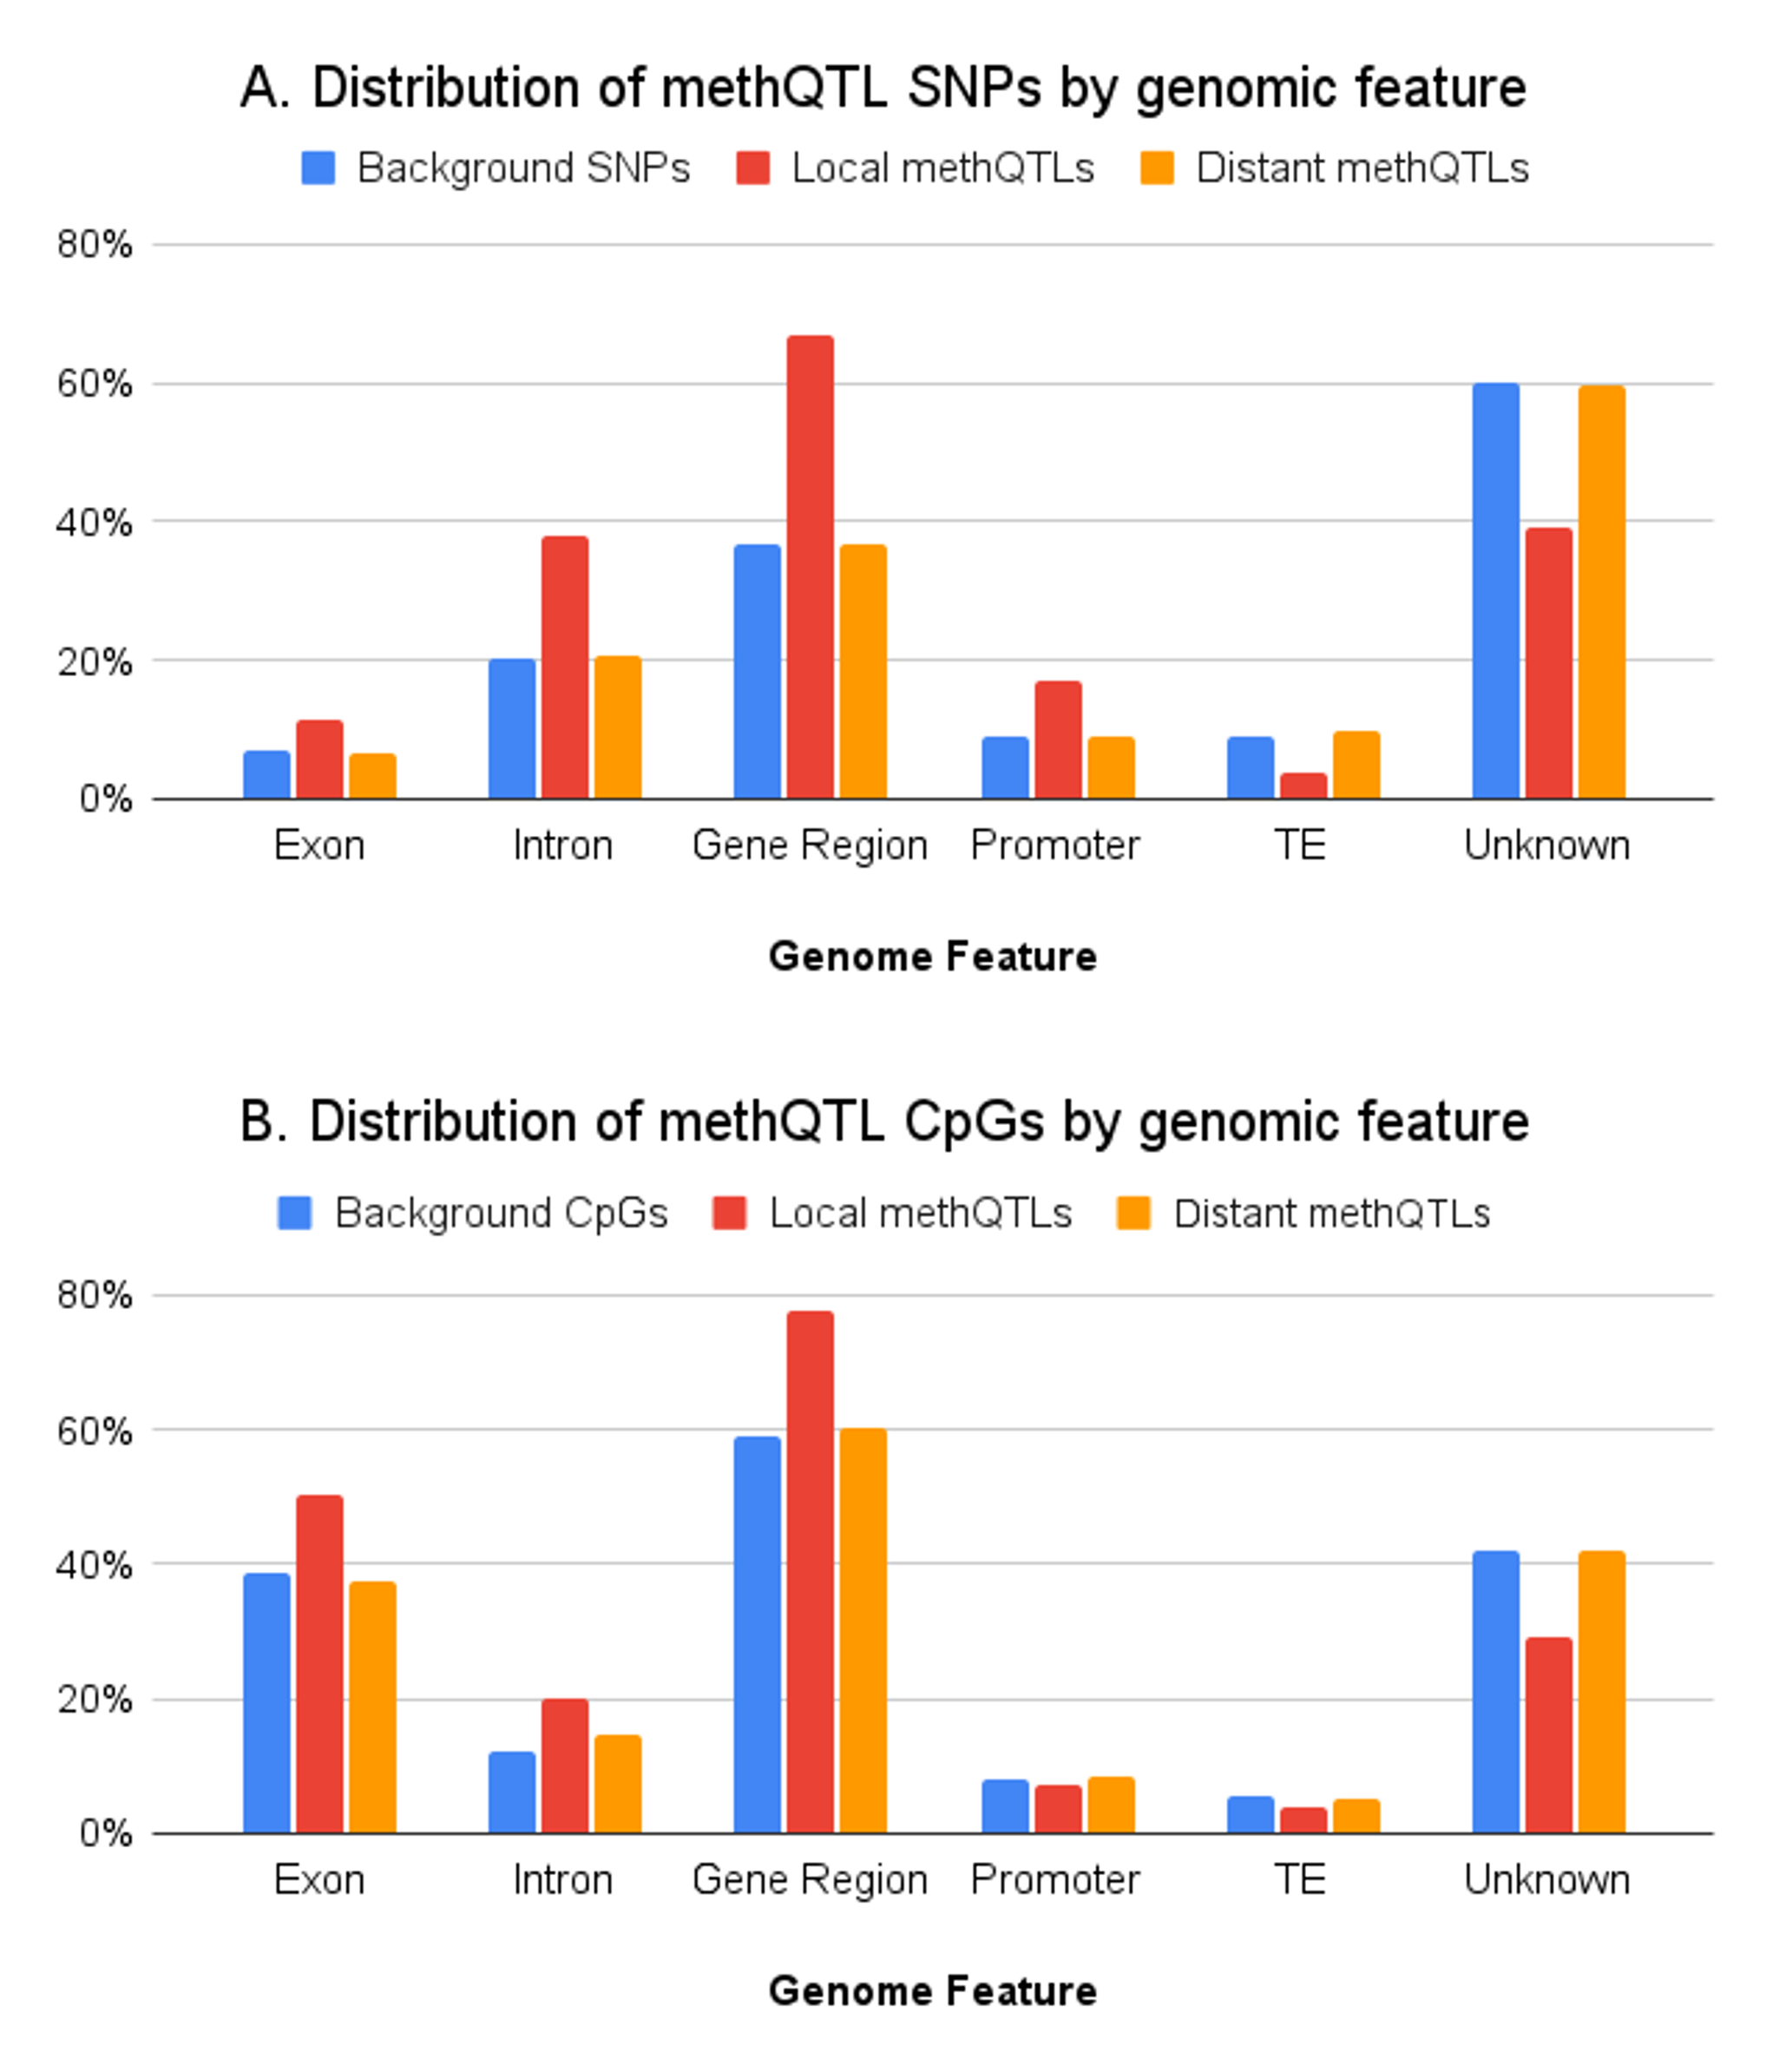
\includegraphics[width=0.7\textwidth,height=\textheight]{../supplemental-files/Supp-09.png}
\caption{\textbf{Supplemental Figure 9:} Comparison of mQTL results that
intersect with the following genomic features: exon, intron, promoter
region (within 2kb of the 5' end of a gene), gene region (genes plus 2kb
upstream and downstream), transposable element, and unknown region of
genome. A) SNPs designated as either local (red, within 50kb) or distant
(orange) mQTLs, compared with the background (blue) of all SNPs used in
the mQTL analysis. B) CpGs associated with either local (red) or distant
(orange) mQTLs, compared to the background (blue) of all CpGs used in
the mQTL}
\end{figure}

\end{document}
